In this chapter we will present in depth the design, manufacturing and functions of the custom measuring board or the Measurement PCB as mentioned earlier in the document. As with every engineering problem, we start by defining the requirements and objectives of the system and later on we focus on the individual parts of it. More specific, it will be shown how the board controls all measurements, in terms of logic and timing, and in addition how each measurement takes place in more details. \par
At this point, it is important to mention that a general goal of the Measurement PCB is to be easily incorporated in a bigger monitoring system, which can have different topologies and parts depending on the specific usage case. Therefore, it is definitely useful to prepare some kind of user manual to make that incorporation as simple and clear as possible. Because this type of material and documentation is not very relevant with the main axes of the thesis, concerning the design and manufacturing of the final device, it will be included as part of the Appendix in the end of the document.

\section{Requirements}
The technical requirements of the Measurement PCB are, of course, driven by the general goals of the project but in the same time should be more specific in terms of numbers and definitions. Generally, as we mentioned earlier in the system's description, the device should be able to accurately measure, on every second, both current and voltage on the output of a PV module as well as a few temperature points. But how do we specifically define which uncertainty level is sufficient enough? What is the desired accuracy for the temperature sensing? What is the range of the measured channels? In order to address these matters and completely describe the technical specifications of the board, we collected all of them in the following list.

\begin{itemize}
  \item Power uncertainty 0.05\% (?check that?)
  \item Temperature sensing accuracy $0.5^oC$
  \item Final measured points of 1Hz
  \item Digital output of the board
  \item Nominal rating at 40V @ 8A (ability to handle peaks to 15A)
  \item Isolated output of the board
\end{itemize}

Below, we make a brief explanation of every one of the above requirements.

\subsubsection{Power uncertainty 0.05\%}
This value is based on results from previous work and experiments on the PV area. (maybe mention IMEC goals or Bert's results?). It is important to understand how this requirement effects the desired accuracy for the current and voltage sensing though. (?check that?)

\subsubsection{Temperature sensing accuracy $0.5^oC$}
Taking into consideration previous work on the area of thermo-electrical PV models and temperature correlation with PV modules' efficiency, we concluded that the accuracy level of half a Celsius degree will be more that efficient.

\subsubsection{Final measured points of 1Hz}
The process of monitoring a system and storing all the logged data usually requires the step of defining the measuring frequency. For that step is important to realize the compromise between plenty of parameters such as the size of stored data, the communication bandwidth needs, the desired "resolution" of the measured points etc. That means that we want to minimize the size of the stored and transferred data, as always, but in the same time have the necessary resolution on the measured points. For the specific case of PV monitoring, taking into consideration the fact that the environmental conditions as well as and the values we want to monitor change rather slowly, we decided that one measured point every second is efficient. This timing standard was also used for the previous research work of the project (Bert) and will keep the comparison and integration of the systems simple. Lastly, it is important to mention that even if the final measured points have a frequency of 1Hz, the sampling for the voltage and current is using averaging and therefore is significantly faster, but we will focus on that in the corresponding chapter.

\subsubsection{Digital output of the board}
The goal of the Measurement PCB, if taken as a black box, is to be able to acquire all the desired data, from different measuring internal circuits and sensors resulting a final output, which contains all the logged values. Therefore, the digital output of the Measurement PCB should be considered more as a consequence of the general board's objective rather than a technical specification of the PCB. But even without that in mind, just in strict technical terms, a digital output is definitely more suitable for this device's scenario.More specific, it would be easier for the control device (second part of the system) to acquire and handle the data. In terms of hardware, this decision is preferable as well, because it keeps the usage of cables to a minimum level (one communication bus for the whole data package comparing to different lines for each analog channel), eliminates the need of external ADC devices and significantly simplifies the way the board is controlled. 

\subsubsection{Nominal rating at 40V @ 8A}
This specification is completely depended on the the type of PV modules used as well as the topology of connections, meaning single PV modules or connected sub-grids. In this particular case, the desired range is up to 40V and 8A in optimal environmental conditions. One very important parameter that we took into consideration when defining the specifications was the fact that in rare cases it is possible to have current peaks up to 15A, which are short in time, but should be the absolute limit of the system. Therefore, the final range that the board should be able to handle is voltages of 40V and currents up to 15A for limited time.

\subsubsection{Isolated output of the board}
The system, as mentioned before, consists of two different parts, one that carries out the measurements and one that handles the acquired data. In the general design philosophy of the Measurement PCB we decided to keep these two parts completely independent, so an intermediate isolation stage was necessary. With that addition, it is guaranteed that in an extreme case of a board failure, given the high values of current peaks, the malfunction could not damage the second part of the system. Last but not least, having the isolation barrier between the two parts contributes also to make the control of the board safer, as it is rather impossible to damage it from the control device's side.

\section{Logic and inputs}
The primary point of the Measurement PCB is the actual measurement of current,voltage and temperature, which make the nature of these inputs the starting point in the process of choosing the board's logic. As all three of the measured inputs are analog values, the need of an analog to digital conversion (ADC) step is clear. There are a few different approaches in the design of such ADC subsystems but we will focus more on them in the next paragraphs. At that point let us take as given the existence of an ADC step, as mentioned above, and try to fill the rest of the design. With the addition of the ADC arises the need of controlling the way the converter operates as well as handling the converted digital result of the conversion. That need is usually fulfilled by a famous electronic component, the microcontroller (mController) which is actually a small computer (SoC) on a single integrated circuit containing a processor core, memory, and programmable input/output peripherals. \cite{mController} More about that crucial part, the process of choosing the right type and the way it controls the board will be described in the next paragraphs.

\subsection{ADC}
There are usually two different lines of action when designing a monitoring system with analog inputs. As mentioned before, it is necessary to include an ADC at some point of the system in order to form the digital form of the measured data. The two different design ideas are:

\begin{itemize}
  \item Digital sensors
  \item Analog to digital converter
\end{itemize}

In the first case, it is possible to use a specific type of sensors which gives back the result of the measured analog value, directly in digital form. That eliminates the need for the extra ADC step, because the result on the output of the sensor is already ready to be handled by any digital system supporting the usual communication protocols. That kind of sensor is being used for the temperature sensing, therefore we do not use extra ADC chips for that measurement.

The second scenario requires the use of a simple ADC component, which can be either integrated in the microcontroller or as an individual IC. The integrated ADC solution is a perfect design approach in case that it is important to keep the final layout simple, minimise the parts' quantity and consequently the cost. In addition it is usually easier, in terms of software development, to use that kind of ADC because there are already written firmware from the microcontroller's manufacturer. The compromises that the designer is forced to accept when using that approach is lower level of accuracy and less bits of resolution. On the other hand, when using an external ADC chip, the designer is able to achieve higher accuracy levels of conversion and in the same time having full control of  the way the converter works, through plenty of parameters and settings. The disadvantages of an external converter are mainly connected with the software development because all parameters and settings will be set by the designer, which can be a complex process requiring experience and know-how. Last but not least, using an external ADC resulting increase of board's size and parts' number, as an extra circuitry will be added.

To summarize the above information, the available options for the current and voltage sensing are two: either a specific sensor for each value, e.g. a current sensor which outputs the data in digital form or an external ADC chip, because the integrated version would be inefficient in accuracy. As highlighted earlier in the report, high level of accuracy is a key element of this project's measurement system. This requirement was not met from the available digital sensors in the market, targeting current and voltage sensing e.g. hall effect sensors.

For this reason, the chosen solution is the use of an external ADC IC, which fulfills all technical requirements, concerning uncertainty and timing. The used IC is the ADS1256 24-bit, very low noise Analog-to-Digital converter from Texas Instruments. The gain error is less than 0.05\% and the range of measurement can be as low as $\pm 78.125$mV which means less effect on the line. Among other benefits of that IC are the serial communication protocols supported, which will make the integration of the board to the system easier and the 4 available input channels, which means that we can measure current and voltage using only one chip. An image of the ADC IC among with a specification table are given below.\\

\begin{figure}[htbp]
	\centering
	\begin{subfigure}[b]{.4\textwidth}
		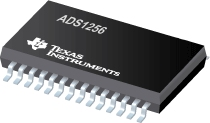
\includegraphics[width=\textwidth]{Chapter_3/ADS1256_chip.jpg}
	    \caption[]{IC}
	    \label{fig:ADS1256_chip}
	\end{subfigure}
    ~
	\begin{subfigure}[b]{.4\textwidth}
		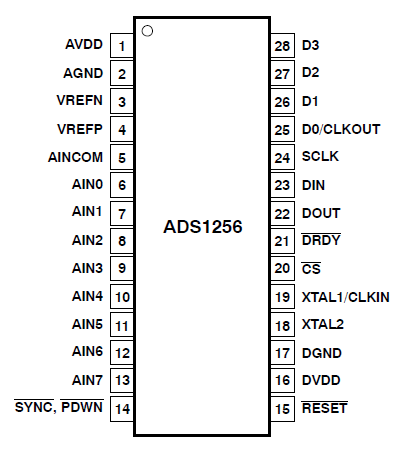
\includegraphics[width=\textwidth]{Chapter_3/ADS1256_pinout.PNG}
	    \caption[]{Pinout}
	    \label{fig:ADS1256_pinout}
	\end{subfigure}
	\rule{35em}{0.5pt}
	\caption{ADS1256 Analog to Digital Converter}
	\label{fig:ADS1256}
\end{figure}


--TABLE OF SPECS ADS1256\\

By observing the above table, we can notice that the ADC has programmable gain meaning we can set the range of the input voltage. It is known that the less effect the Measurement PCB causes to the power line of the PV module the better efficiency we achieve. Therefore, from the available gain values we chose the biggest one, PGA:64, resulting the minimum voltage range of just $\pm 78.125$mV. The only thing left is to scale the voltages we area interested to measure down to that range and feed them in the input channels of the ADC. More details on the circuitry for the measurement are given in the next sections.

\subsection{mController}
Next step of the design process, after the decision on the preferable ADC solution, is choosing the control unit of the board. All tasks that this particular component is requested to address are given in the following list:

\begin{itemize}
    \item Configuration of ADC, RTC (not mentioned before!!), Temperature sensors
    \item Control the ADC and get the current, voltage measurements
    \item Control the Temperature sensors and get the temperature points
    \item Control the RTC and get the current time-stamp
    \item Handle the board's clock signals, using the RTC's 1Hz pulse function
    \item Gather all logged data from current second and construct a complete data package
    \item Transfer the data packages to the control device
    \item Control user interaction tasks such as LED indicators and buttons
\end{itemize}

By observing the above list we can easily see the important role of the microcontroller, as the "brain" of the whole Measurement PCB. The available component options in market, cover once again a wide range of ICs with different specifications, architecture and supported peripherals and features. A few of the well known microcontroller fabrication "houses", targeting in the are of this project, are among others Texas Instruments, Altera, Maxim Integrated, Microchip and Atmel, with the last two companies being the most popular option. In order to decide which device is more suitable for this task, we have to describe the main requirements that are crucial to the board's functionality and efficiency:

\begin{itemize}
    \item Enough I/O ports to handle the different components of the board
    \item Support of the common protocols for communication between the components, such as I2C, SPI and 1-Wire
    \item Support of interrupts, in order to handle the 1Hz clock pulse from RTC
\end{itemize}

Furthermore, there are a few important factors that although are not necessary for the development of the board will significantly improve the design and mostly decrease the required development time. Among them are the following:

\begin{itemize}
    \item Ease of software development through high level programming and libraries
    \item Development tools such as sophisticated IDEs and general purpose development boards
    \item Documentation material and support through manufacturer's services, forums etc
\end{itemize}

Taking all the above parameters into consideration and after searching the available options in market, we decided to narrow our choices to the family of AVR microcontrollers from Atmel. There are a few processors from that group that fulfill all the desired specifications mentioned before, so the last step is to conclude to the final device selection. In that point it would be fair to mention the existence of a slightly different approach to the whole microcontroller programming and development area, called Arduino.

Arduino is an open-source platform used for building electronics projects and combines the physical programmable development board option with a complete IDE, used to write and upload code to the microcontroller. There are plenty different models of Arduino boards, using different microcontrollers and components depending on the board's target area. The most suitable board for this project, capable of simple and fast prototyping, is called Arduino Uno and is based on the microcontroller Atmega328 of AVR series, from the company Atmel.\\

\begin{figure}[htbp]
	\centering
		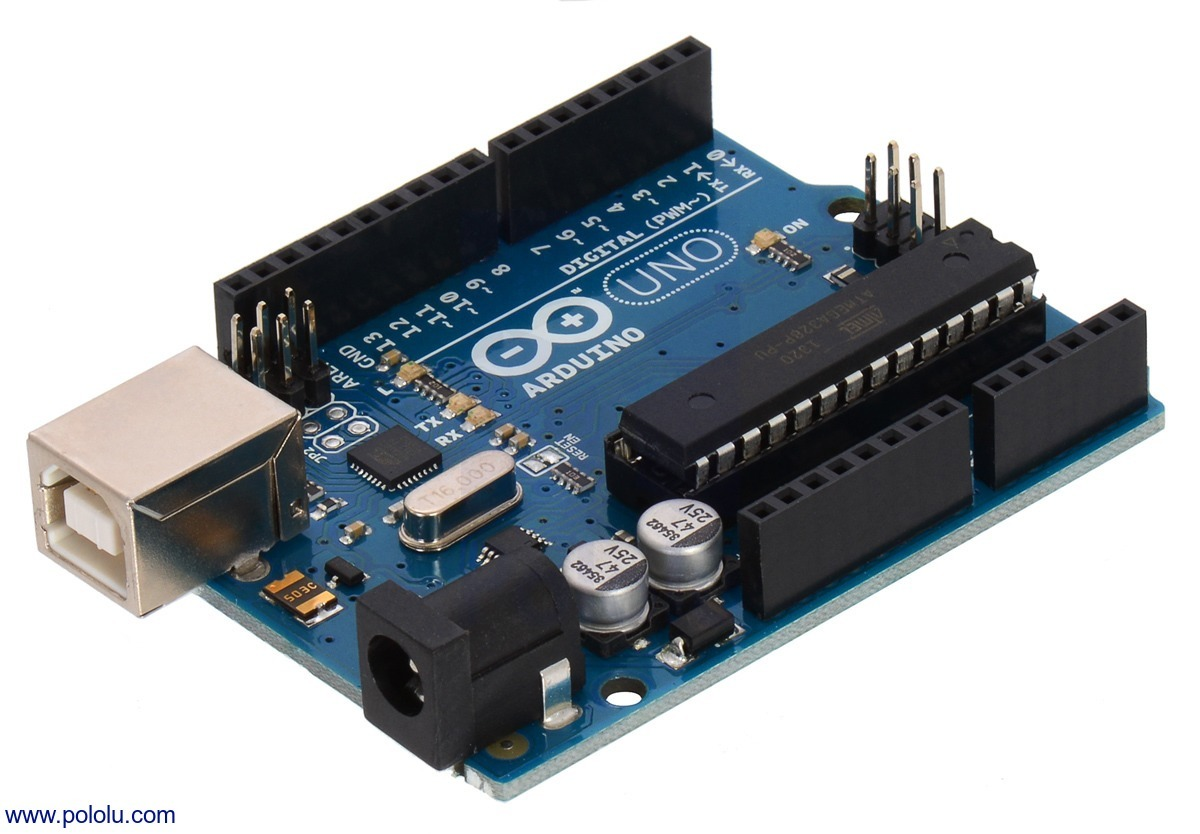
\includegraphics[width=0.7\textwidth]{Chapter_3/arduinoUno.jpg}
		\rule{35em}{0.5pt}
	\caption{Arduino Uno board}
	\label{fig:arduinoUno}
\end{figure}

So far, we have mentioned a wide spectrum of microcontroller solutions; so what makes the Arduino option so special? To answer that question, we have collected the main advantages of the Arduino platform in the following list:

\begin{itemize}
    \item Inexpensive development board, excellent for prototyping
    \item Supports all previously mentioned hardware requirements (I/O ports, protocols, interrupts etc)
    \item Free IDE for PC, which communicates with the board through USB
    \item Growing on-line community for support during development
    \item Huge amount of available code libraries for functions, peripherals etc
    \item Excellent documentation
    \item Open source project, highly customisable and expandable
\end{itemize}

At this point it would be crucial to clarify the following. Although Arduino boards are perfect for prototyping and development, they cannot be considered acceptable as a final option, at least for this project objectives. Their size and cost is a serious problem because we are designing a product with specific needs, which require permanent and size respecting solutions, thus no flexible development board are suitable. The way to keep all the advantages of Arduino but still achieve the goals of size and cost is by using the Arduino for prototyping and when designing the final board only use the atmega microcontroller as standalone IC. With a few accompanying components for the microprocessor's circuitry, it can support all the functions of a complete Arduino board, while enormously reducing the board's size and parts' list.\\

\begin{figure}[htbp]
	\centering
	\begin{subfigure}[b]{.4\textwidth}
		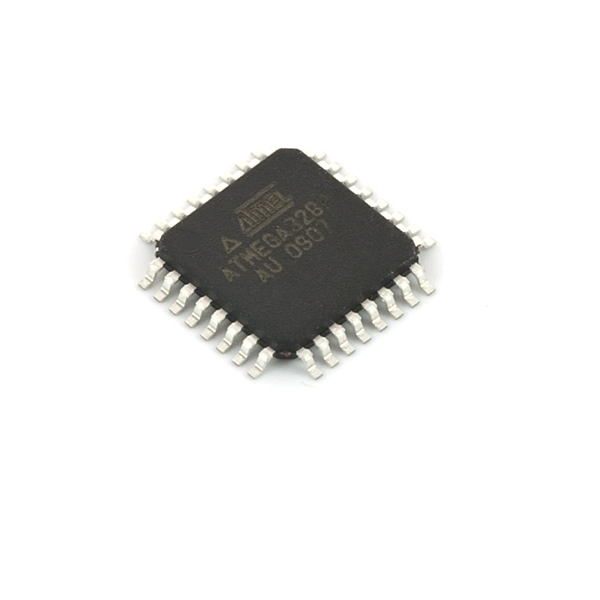
\includegraphics[width=\textwidth]{Chapter_3/atmega_chip.jpg}
	    \caption[]{IC}
	    \label{fig:atmega_chip}
	\end{subfigure}
    ~
	\begin{subfigure}[b]{.4\textwidth}
		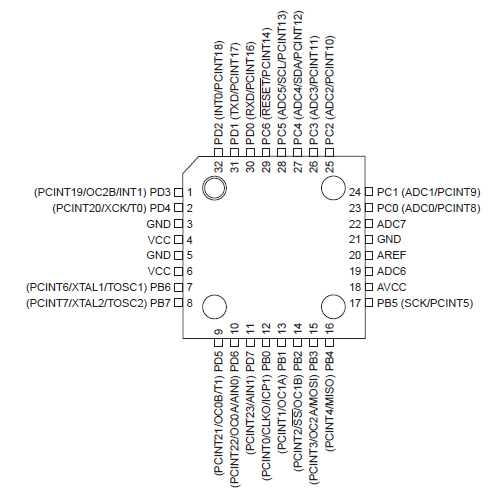
\includegraphics[width=\textwidth]{Chapter_3/atmega_pinout.PNG}
	    \caption[]{Pinout}
	    \label{fig:atmega_pinout}
	\end{subfigure}
	\rule{35em}{0.5pt}
	\caption{Atmega328 microcontroller}
	\label{fig:atmega}
\end{figure}

The most important specifications of the Atmega microcontroller are given in the table below:\\

--TABLE OF SPECS for atmega328\\

\section{Electrical measurements}
In this section we will analyze how the measurements of current and voltage on the output of the PV module are carried out. Both of these measurements need to be transformed to a voltage signal readable, in terms of value range, from the ADC chip. That means that we need to scale the measured voltage down to $\pm 78.125$mV. For the voltage sensing the easiest, yet quite accurate way to get the measurement is by using the method of voltage divider, as described more in depth in the corresponding paragraph. Concerning the current sensing, we do not have any voltage to measure to start with. For this reason, as we have chosen not to work with digital current sensors, we can use the simple, yet precise, method of shunt resistor. To get the value of the current, using this approach, a shunt resistor is added in line to the measured circuit trace, causing a voltage drop across it, which can be later on measured by the ADC. More details about the current sensing circuitry in the corresponding paragraph below.

An abstract representation of the circuit used for the electrical measurements on the output line of the PV module is shown in the next figure.\\

--IMAGE OF THE ABSTRACT CIRCUIT (voltage and current meter circles in the lines)\\

Last but not least, before designing the measuring circuit it is important to define the nominal operation values of the PV output. The type of module that we targeted in this project, as described in the system description chapter, is giving an output voltage of 40V DC with current flow at 8A. Nevertheless, it is possible in a few rare cases to have current peaks up to 15A, which means that the measuring circuit should be able to handle that amount of current flow, at least for a limited time period.

\subsection{Voltage}
Let us start with the output voltage of the PV module, which is 40V DC. This voltage needs firstly to be scaled down to 78mV and after that fed to one input channel of the ADC. In order to achieve this scaling, we will use the simple method of voltage divider, as shown in the figure below. One can notice that the voltage that the PV module outputs is marked as $V_p$ and the one measured by the ADC as $V_m$.\\

--IMAGE OF VOLTAGE DIVIDER\\

There could be some concerns about the power consumption with that method, but in the design process we chose the parts’ values in order to minimize the current flow (less than $75\mu$A) through the divider and consequently the power consumption.

For the calculations of the resistors we need to take into consideration:

\begin{itemize}
    \item the resistors' ratio for the desired scaling
    \item the total resistance of the whole divider
\end{itemize}

Also, we have to adjust the resistors' values corresponding to the differential input impedance of the ADC, because the actual circuit is closer to the slightly altered version shown in the figure below.\\

--IMAGE OF VOLTAGE DIVIDER WITH R of ADC\\

We start the calculations with the differential input impedance $R_{IN}$, of the ADC, which is given by the datasheet as an $80M\Omega$ resistor, when an internal buffer is enabled. In order to eliminate the effect of that impedance, the $R_2$ should be a few scales smaller than $R_{IN}$, in order to minimize the current escaping from the $R_2$ to the ADC pins.

We decided to scale down at least 10000 times, so $R_2$ should be at maximum:

\begin{equation}
R_2 \ll \left( R_{IN} \over 10000 \right) = 8k\Omega
\label{eqn:maximum_R2}
\end{equation}

Because of that big scale difference between $R_2$ and $R_{IN}$, the influence of the second will be almost invisible, therefore it is sufficient to completely ignore $R_{IN}$ for the calculations. The measured voltage $V_m$ and the current $I_m$ of the voltage divider's branch, are given by the following equations:

\begin{equation}
V_m = I_m \cdot R_2
\label{eqn:Vm_general}
\end{equation}

\begin{equation}
I_m = \left. V_p \over R_1 + R_2 \right.
\label{eqn:Im_general}
\end{equation}

The expression \ref{eqn:Vm_general}, because of the \ref{eqn:Im_general} can be written as:

\begin{equation}
V_m = \left. V_p \over R_1 + R_2 \right. \cdot R_2 \Leftrightarrow R_1 = \left. V_p \cdot R_2 \over V_m \right. - R_2
\label{eqn:Vm}
\end{equation}

In that point we had to experiment with different values of $R_2$ and $R_1$, which we could find on market with the desired precision. The final decided value of $R_2$ was $1k\Omega$, so the $R_1$ is calculated from the expression \ref{eqn:Vm}, as shown below. 

\begin{equation}
R_1 = \left. 40 \cdot 1000 \over 78.125 \times 10^{-6} \right. - 1000 \Rightarrow R_1 \cong 511820\Omega
\label{eqn:R1_calculation}
\end{equation}

The closest and safest option for $R_1$ was $560k\Omega$. Knowing the values of the resistors, we can
calculate the current on the divider with the expression \ref{eqn:Im_general}:

\begin{equation}
I_m = \left. 40 \over 560000 + 1000 \right. \Rightarrow I_m = 71.3\mu A
\label{eqn:Im_calculation}
\end{equation}

And after that, we can also calculate the final voltage range on the ADC from the expression \ref{eqn:Vm_general}, as follows:

\begin{equation}
V_m = 71.3 \times 10^{-6} \cdot 1000 \Rightarrow V_m = 71.301mV
\label{eqn:Vm_calculation}
\end{equation}

Concerning the power of the resistors, we can calculate:

\begin{equation}
\begin{split}
P_{R_1} = I_m^2 \cdot R_1 \Rightarrow P_{R_1} = 2.85mW \\
P_{R_2} = I_m^2 \cdot R_2 \Rightarrow P_{R_2} = 5.08\mu W
\end{split}
\label{eqn:Resistor_power}
\end{equation}

The final values of the resistors were chosen with a big safety factor concerning power while respecting the available market options.\\

\begin{center}
\begin{tabular}{ c c c c } 
 Resistor & Value & Tolerance & Power \\ \hline
 $R_1$ & $560k\Omega$ & 0.1\% & 250mW \\ 
 $R_2$ & $1k\Omega$ & 0.1\% & 125mW \\ 
\end{tabular}
\end{center}

\subsubsection{Internal buffer issue}
After assembling the boards and experimenting with the ADC, we faced some problems with unstable behavior of the converter, when the input buffer was enabled. The solution was to disable that buffer, with the consequence of really smaller value of input impedance, at $4.7k\Omega$, as given by the datasheet. At first we were concerned about this change but as the following calculations prove, this was not a real problem and the board worked perfectly.

The parallel resistance $R_par$ of the combination of $R_2$ and $R_{IN}$ can be calculated:

\begin{equation}
R_{par} = \left. R_2 \cdot R_{IN} \over R_2 + R_{IN} \right. \Rightarrow R_{par} = 825\Omega
\label{eqn:R_parallel}
\end{equation}

So, the total resistance of the divider's branch will be:

\begin{equation}
R_{total} = R_1 + R_{par} \Rightarrow R_{total} = 560825\Omega
\label{eqn:R_total}
\end{equation}

resulting a new current:

\begin{equation}
I_m = \left. 40 \over 560825 \right. \Rightarrow I_m = 71.323\mu A
\label{eqn:Im_new_calculation}
\end{equation}

The difference with the previously calculated current is almost invisible. Lastly, we can calculate
the new voltage range that the ADC will “see” from the expression \ref{eqn:Vm_general}, which is 59mV. This value is inside the ADC voltage range as predicted but slightly smaller than initially calculated, meaning we do not use the full range of 78mV and consequently the full resolution capabilities. On the other hand, with this setting of buffer disabled, the board is giving good and stable measurements, so we decided to keep the system as is. At this point it would be fair to mention that this change will be no results calculation errors carried to the final measured data because of the calibration process, which will be discussed later on in the report. A possible alternative could be a smaller $R_2$ and $R_1$, but with the same ratio (???check that???).

\subsection{Current}
The second electrical measurement that the board will carry out is the current sensing. More specific we are interested to measure the current at the output of the PV module, flowing towards the DC-DC and the grid. As mentioned before, because of the desired accuracy and the nature of the panel's output, we decided not to use  magnetic field sensors but implement the simple method of the shunt resistor. There are three basic techniques used for sensing current using shunt resistors \cite{current_sense_Linear}, which are:

\begin{itemize}
    \item Low side sensing
    \item High side sensing
    \item Full range sensing
\end{itemize}

The third method is useful in scenarios when the current can flow in both directions, which is not the case for this project. In effect, we will focus only to the first two methods which differ in the position that the shunt is placed inside the circuit. 

\subsubsection{Low side current sensing}
In the low side sensing, the current is measured in the ground return path of the power connection to the monitored load, as shown in the figure -FIGURE NUMBER-. As mentioned above, the current should flow only in one direction.\\

--IMAGE OF LOW SIDE SENSING CIRCUIT\\

The main advantages of this method are:

\begin{itemize}
    \item Low voltage on input (common mode)
    \item Ground referenced output voltage
    \item Easy design using single-supply
\end{itemize}

On the other hand, there are a few disadvantages when using low side current sensing:

\begin{itemize}
    \item Load not directly connected to ground
    \item Load activated by accidental short at ground end load switch
    \item In case of short, no detection of high load current
\end{itemize}

\subsubsection{High side current sensing}
When using this method the current is sensed in the supply path of the power connection to the monitored load. Once again, the current should flow only in one direction, as shown in the figure -FIGURE NUMBER-.\\

--IMAGE OF HIGH SIDE SENSING CIRCUIT\\

The high side current sensing benefits are:

\begin{itemize}
    \item Load is directly grounded
    \item Load not activated by accidental short at power connection
    \item In case of short, high load current detection is possible
\end{itemize}

On the contrary, when the designer is using this current sensing method he has to deal with a few drawbacks, such as:

\begin{itemize}
    \item High voltage on input (common mode)
    \item Output needs to be level shifted down to system operating voltage levels
\end{itemize}

Given the nature of the PV module output and the project's requirements, we concluded that the most appropriate technique for the current measurement is the low side sensing. With this in mind, the circuit used for the current measurement will be as shown in the figure -FIGURE NUMBER-.\\

--IMAGE OF CURRENT SENSING CIRCUIT\\

For the calculation of the shunt value, we start from the desired measured voltage $V_{sh}$ and specifically the ADC input range of 78mV. So, given that $V_{sh} = 78.125mV$ we can proceed with the calculation of the shunt resistor $R_{sh}$

\begin{equation}
R_{sh} = \left. V_{sh} \over I \right.
\label{eqn:Rs_general}
\end{equation}

In order to make the system able to handle the current peaks, we will work with the maximum current value $I_{max}=15A$, and the expression \ref{eqn:Rs_general} will give us the value of the shunt.

\begin{equation}
R_{sh} = \left. V_{sh} \over I_{max} \right. \Rightarrow R_{sh} = \left. 78.125 \times 10^{-3} \over 15 \right. \Rightarrow R_{sh} = 0.00521\Omega
\label{eqn:Rs_calculation}
\end{equation}

For safety reasons, we choose the lowest option close to that value which is $R_{sh} = 0.005\Omega$

Next step is calculating the power specification of the shunt, again for the worst case scenario of $I_{max}$

\begin{equation}
P_{sh} = I_{max}^2 \cdot R_{sh} \Rightarrow P_{sh} = 15^2 \cdot 0.005 \Rightarrow P_{sh} = 1.125W
\label{eqn:Ps_calculation}
\end{equation}

As always, we search for the closest option that still is on the safe side, concerning the power of the shunt too. For this reason the final choice for the shunt resistor is:

\begin{center}
\begin{tabular}{ c c c c } 
 Resistor & Value & Tolerance & Power \\ \hline
 $R_{sh}$ & $0.005\Omega$ & 0.1\% & 2W \\ 
\end{tabular}
\end{center}

In conclusion of everything we have discussed on that section about the electrical measurements, we can design the final circuit as shown in figure -FIGURE NUMBER-.\\

--IMAGE OF WHOLE CIRCUIT\\

At that point we have to clarify a few details concerning this circuit. First of all, one can notice that there are two voltage dividers instead of the single one we mentioned in the voltage sensing paragraph. The second divider is used in order to have a better image concerning the power losses caused by the shunt and it is completely optional. That means we designed the final PCB with the option to completely disable the second voltage divider, or even both of them if desired, by adjusting the position of two jumper pins. More on these options will be discussed in the corresponding chapter of the final PCB.

Second point that needs to be noted is the addition of a safety fuse. As shown in the circuit, there is an overcurrent fuse added in series with the return power line. More specific, in case there is an unexpected current peak higher than 15A, will cause the fuse to burn and consequently break the connection. In this way, the system will protect itself, avoiding long period of high current flow. It is important to notice that the fuse is placed just before the return connection with the PV module, in order to protect the system from overcurrent in any of the circuit's branches.

\section{Temperature}
One interesting part of this PV monitoring system is the addition of temperature measurement, as it proved to be a significant factor when examining the efficiency of a PV module. The specifications of that measurement are:

\begin{itemize}
    \item Temperature accuracy $0.5^oC$
    \item Up to 20 measuring points per device
    \item As less connections and cables as possible
    \item Convenient sensor package, easy to mount and weather resistant
\end{itemize}

The available options for temperature measurement were once again plenty, including thermocouples, thermistors and  resistance temperature detectors (RTD). Nevertheless, the 20 measuring point requirement helped us narrow our choices, because any analog solution would require huge amount of cabling. For this reason, the digital sensors, and especially the ones that can be wired to a single data line, were the only acceptable option.

The final solution we chose, after searching the available options in market, was the DS18B20 digital, 1-Wire temperature sensor. The big advantage of that type of sensor is that it requires only one data bus for all the sensors, as noted before, which means that we will only use one pin of the microcontroller to get all 20 temperature measurements. Additionally, the accuracy is inside the required range and the device package (3TO-92) is really convenient for the gluing application on the back side of the PV module.\\

\begin{figure}[htbp]
	\centering
	\begin{subfigure}[b]{.4\textwidth}
		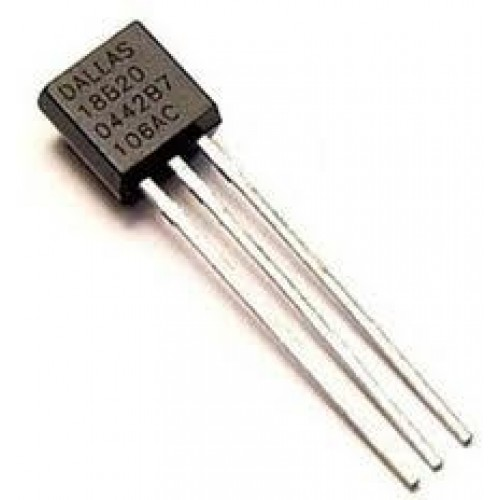
\includegraphics[width=\textwidth]{Chapter_3/DS18B20_chip.jpg}
	    \caption[]{IC}
	    \label{fig:DS18B20_chip}
	\end{subfigure}
    ~
	\begin{subfigure}[b]{.1\textwidth}
		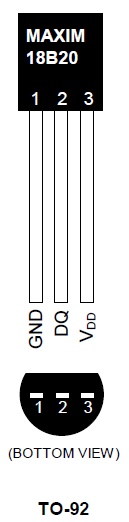
\includegraphics[width=\textwidth]{Chapter_3/DS18B20_pinout.PNG}
	    \caption[]{Pinout}
	    \label{fig:DS18B20_pinout}
	\end{subfigure}
	\rule{35em}{0.5pt}
	\caption{DS18B20 temperature sensor}
	\label{fig:DS18B20}
\end{figure}

The basic specifications of the DS18B20 sensor are given in the table -NUMBER OF TABLE-.\\

--TABLE OF SPECS for the DS18B20 sensor\\


\section{Time}
This part of the board has a double purpose, serving two different goals. More specific, the timing objectives can be summed to the followings:

\begin{itemize}
    \item Precise 1Hz clock signal for the measurements's timing
    \item Timestamp generation for each measurement
\end{itemize}

Starting with the 1Hz clock, there are a few different techniques used for clock generation. The most popular options are:

\begin{itemize}
    \item Analog circuits (RLC circuits or timer ICs with RC circuitry)
    \item Crystal and microcontroller
    \item Real Time Clock ICs (RTC)
\end{itemize}

The first option, of analog design circuits is not only complex to design but most importantly not even close to the precision level we target in the project. The second alternative of using an external crystal, with a specific frequency, combined with the microcontroller gives better results in terms of precision but again not in the desired level. In addition, this design approach would add an extra task for the processor to handle resulting even more complex programming concerning timing and delays.

So, the optimal solution seems to be the use of RTC chips, which not only could produce high precision clocking signals but in the same time help the development with useful functions. After searching the market for the available options, we concluded to the DS3234 RTC from Maxim Integrated Products. This IC fully covers all mentioned requirements and even provide extra tools to increase the efficiency of the board, such as timestamp generation, leap year compensation, SPI bus communication and Arduino libraries).\\

\begin{figure}[htbp]
	\centering
	\begin{subfigure}[b]{.4\textwidth}
		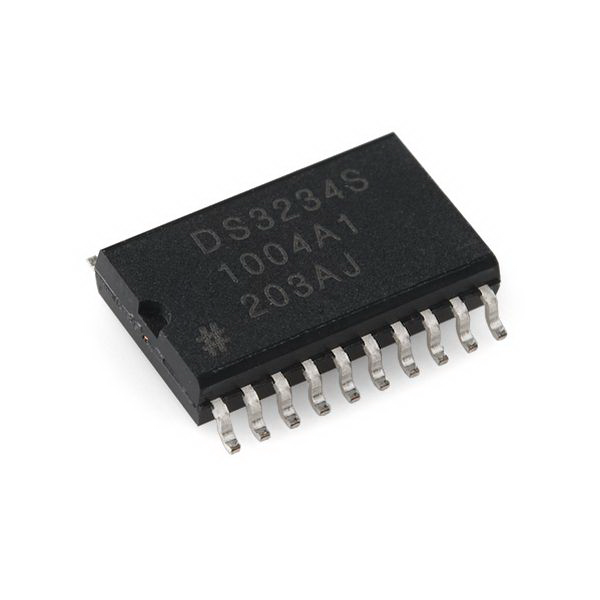
\includegraphics[width=\textwidth]{Chapter_3/DS3234_chip.png}
	    \caption[]{IC}
	    \label{fig:DS3234_chip}
	\end{subfigure}
    ~
	\begin{subfigure}[b]{.4\textwidth}
		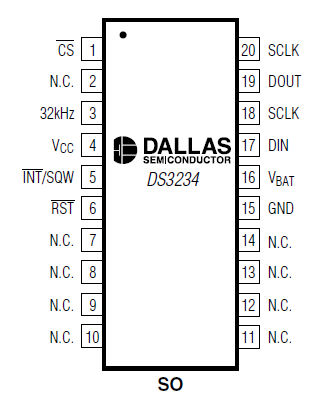
\includegraphics[width=\textwidth]{Chapter_3/DS3234_pinout.png}
	    \caption[]{Pinout}
	    \label{fig:DS3234_pinout}
	\end{subfigure}
	\rule{35em}{0.5pt}
	\caption{DS3234 Real Time Clock}
	\label{fig:DS3234}
\end{figure}

The basic specification of the DS3234 real time clock are given in the table -NUMBER OF TABLE-.\\

--TABLE OF SPECS for the DS3234 RTC\\

\section{Isolation}
The last important requirement that we have not addressed in depth yet is the isolation of the board's output. This is a very common guideline when a system has parts with different scales of current, voltage or frequencies. In particular, this intermediate isolation layer between the two parts of the system has a double purpose:

\begin{itemize}
    \item Protect the control device from any malfunction that may occur in the Measurement PCB side. Keep in mind that this board is handling high values of current and therefore any failure could be harmful if transferred outside of the board.
    \item Protect the Measurement PCB from the control device, in case of mistake or failure such as wrong connection, different logic level signals etc.
\end{itemize}

This isolation layer should be able to address two different tasks, firstly provide isolated DC power to the board from the control device and also completely isolate the communication and signal buses between these two sides. Taking care of these tasks consequently means full isolation of the Measurement PCB, as required from the initial project goals.

\subsection{Isolated power supply}
The Measurement PCB is powered from the control device, with 5V DC power line. In order to isolate this rail and actually design an isolated power supply to drive the board, we decided to use an isolated DC-DC converter. These converters are required in a broad range of applications including power metering, industrial programmable logic controllers (PLCs), industrial automation and they are often used to provide:

\begin{itemize}
    \item galvanic isolation
    \item improve safety
    \item enhance noise immunity
    \item multiple output voltage rails
\end{itemize}

In this particular design we are using the ADuM5000 2.5 kV, Isolated DC-to-DC Converter from Analog Devices, as shown in the figure -FIGURE NUMBER-.\\

\begin{figure}[htbp]
	\centering
	\begin{subfigure}[b]{.4\textwidth}
		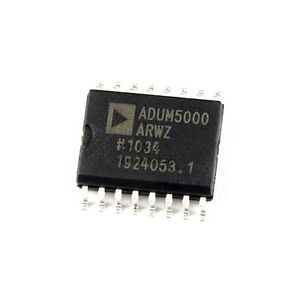
\includegraphics[width=\textwidth]{Chapter_3/ADUM5000_chip.jpg}
	    \caption[]{IC}
	    \label{fig:ADUM5000_chip}
	\end{subfigure}
    ~
	\begin{subfigure}[b]{.3\textwidth}
		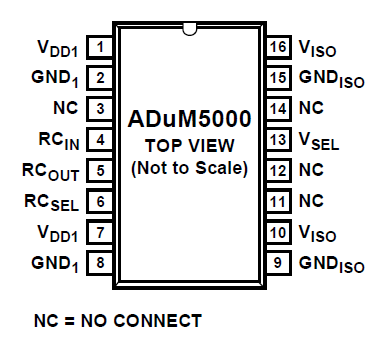
\includegraphics[width=\textwidth]{Chapter_3/ADUM5000_pinout.PNG}
	    \caption[]{Pinout}
	    \label{fig:ADUM5000_pinout}
	\end{subfigure}
	\rule{35em}{0.5pt}
	\caption{ADUM5000 DC-DC isolated converter}
	\label{fig:ADUM5000}
\end{figure}

It is often for this kind of converters to get high temperature because of the power switching, so one concern we had about this IC was the heat generation possible issue. But in this particular case, we thoroughly tested the chip when the board was logging data for long periods of time and the temperature levels were completely acceptable.

The basic specification of the ADum5000 converter are given in the table -TABLE NUMBER-.\\

--SPECS TABLE for ADum5000\\

\subsection{Signal isolation}
In addition to the isolated power supply, the board needs to facilitate a communication isolation stage. More specific, except from the power lines that are fed through the DC-DC converter, the signals that need isolation are:

\begin{itemize}
    \item Microcontroller's reset pin
    \item Data ready flag pin
    \item I$^2$C bus (NOT MENTIONED BEFORE ???check that???)
\end{itemize}

For the signal isolation we searched the available options in the market and concluded that the most suitable option is the MAX14850 six-Channel digital isolator from Maxim Integrated, shown in the figure -FIGURE NUMBER-.\\

\begin{figure}[htbp]
	\centering
	\begin{subfigure}[b]{.3\textwidth}
		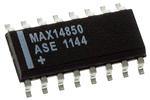
\includegraphics[width=\textwidth]{Chapter_3/MAX14850_chip.jpg}
	    \caption[]{IC}
	    \label{fig:MAX14850_chip}
	\end{subfigure}
    ~
	\begin{subfigure}[b]{.3\textwidth}
		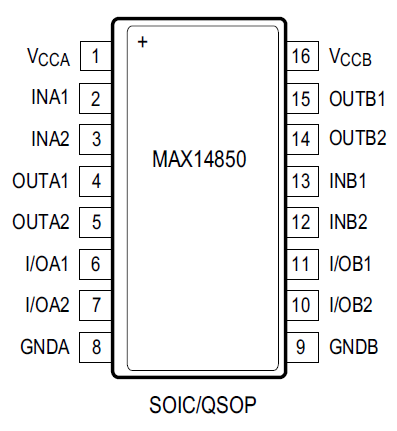
\includegraphics[width=\textwidth]{Chapter_3/MAX14850_pinout.PNG}
	    \caption[]{Pinout}
	    \label{fig:MAX14850_pinout}
	\end{subfigure}
	\rule{35em}{0.5pt}
	\caption{MAX14850 6-Channel Digital Isolator}
	\label{fig:MAX14850}
\end{figure}

The advantages of MAX14850 isolator are not limited in the capability of single digital signal isolation, but are including two bidirectional open-drain signal paths. This specification means that this channels can be used to isolate communication buses based on common protocols, such as SPI and I$^2$C, which makes the specific chip ideal for our project.

Furthermore, independent 3.0V to 5.5V supplies on each side of the isolator make it suitable for use as a level translator. As a result, we can use the MAX14850 chip not only as a signal isolator but also as a logic level shifter. Given that key characteristic of the board, we can connect the Measurement PCB, in the control side, with a device based on either of the two logic levels (e.g. an Arduino Uno board runs usually on 5V logic in contrast to an Raspberry Pi board which uses 3.3V).

The basic specifications of the MAX14850 isolator are given in the table -TABLE NUMBER-.\\

--SPECS TABLE for MAX14850\\

\section{PCB Design}
This section is dedicated to the design and manufacturing process of the final measuring PCB. Among the subjects that will be discussed are a basic introduction to the PCB technology, the steps of designing and prototyping the PV Measurement board and in the end the actual testing.

\subsection{Introduction}
Printed circuit boards (PCBs) are by far the most common method of assembling modern electronic circuits and creating functional pieces of hardware \cite{AD_BasicLinearDesign}. Comprised of a sandwich of one or more insulating layers and one or more copper layers which contain the signal traces and the powers and grounds, the design of the layout of printed circuit boards can be as demanding as the design of the electrical circuit.

The term "Printed Circuit Board" (PCB) has been loosely used to describe board fabricated with a variety of methods. \cite{TorontoUNI_GuideToPCB} The most common way of manufacturing big quantities of boards, e.g. for commercial high quality production line, is based on photolithography. In particular, the undesired copper regions are defined optically using a photolithograpic mask, which explains why traditional PCBs are considered to be "printed", and next are chemically etched away from the copper substrate. This method, often with minor alterations such as using the toner's ink material of a laser printer instead of the photosensitive mask, has become more accessible to smaller designers and even hobbyists during the last years, resulting an huge increase in designs, ideas and techniques. Lastly, there is also an alternative method of creating PCBs by removing the unwanted copper areas using a purely mechanical process, known as milling. An example of the layering pattern of a common PCB is given in the figure -FIGURE NUMBER- below.\\

--IMAGE OF PCB LAYERS\\

The creation of a functional PCB requires a few steps, as shown in the figure -FIGURE NUMBER-. First of all, the designer has to design a draft version of the system and create a prototype. Prototyping in general includes circuit development using breadboards, simple wired connections or even simple boards made by the designer in a more "Do It Yourself" (DIY) approach. After creating the first prototypes, the designer is able to test the system and further develop both the hardware and the software used. This iteration of prototyping, testing, changing the design and assemble a prototype again can take place multiple times until the desired result is reached. At that point, when the collection of all the working prototypes functions and addresses the system's goals (or at least a majority of them), the designer can proceed to the next stage. This stage consists of the creation of the final schematic of the circuit and the design of the final board's physical layout. Only after these two steps, it is possible to manufacture the final board through a fabrication "house" or sometimes even in a small laboratory e.g. in a university. Last step of the board creation, before the testing stage, is the physical assembly and soldering of all the components used such as ICs, resistors, capacitors, connector etc.\\

--IMAGE OF STEPS FOR PCB DESIGN\\

MAYBE ADD HERE THE COMMON PCB ISSUES/NOTES??\\

\subsection{Initial Design and Prototyping}
In the next paragraphs, we will discuss how the design process of the measuring system started to take shape, including the initial design of the circuit for both the electrical measurements and the temperature sensing as well as the development and testing of the prototypes and modules. 

\subsubsection{Electrical measurements}
The core of the measuring system, as stated before, is the electrical measurement of the voltage and current on the PV module output. Therefore it makes perfect sense to start from this point and describe how the first demo board with the measuring circuitry was designed. So far we have discussed the basic parts of this system, which are:

\begin{itemize}
    \item Atmega328 mController for the board's control
    \item DS1256 ADC for the analog values measurement
    \item Voltage dividers for voltage sensing
    \item Shunt for current sensing
\end{itemize}

First important point concerning the electrical measurements demo board is the fact that we did not include the microcontroller into the design. More specific, we decided to focus completely on the measurements themselves, which lead us to use externally an Arduino Uno board featuring the same microcontroller as planned. So, for this reason we only added the necessary connection points, in order to be able to achieve communication between the Arduino board and the ADC in the demo board.

Having the microcontroller part clarified, we can proceed with the design of the actual measuring circuit. As described before, it consists of the ADC, the main current path from the PV module output to the board's output, the two voltage dividers and the shunt for voltage and current sensing respectively.

In addition, it is very common for the majority of ICs to require extra electronic components such as resistors and capacitors to support their operation. Usually the capacitors are used to decouple (also mentioned as bypass) the power and ground traces or even input channels. This norm applies to all of the chips used in the demo board and therefore you can easily notice a big number of capacitors and a few resistors, used in every part of the circuit, as requested by each component's datasheet.

One more point to mention concerning the schematic of the circuit is the fact that the ADC chip requires three different voltage levels to operate, as documented in the part's datasheet. More specific it needs:

\begin{center}
\begin{tabular}{ l l l } 
 Voltage & Pin & Function \\ \hline
 5V & AVDD & Analog power supply \\ 
 3.3V & DVDD & Digital power supply \\
 2.5V & VREFP & Positive reference input \\ 
\end{tabular}
\end{center}

For the first two voltage levels, there are no strict requirements as they are power supply lines and therefore we can simply use the corresponding Arduino Uno board's pins to directly provide them to the chip. On the other hand, the 2.5V voltage is used for the conversion as voltage reference, meaning it is critical to be precise and stable. For this reason, it is important to use the appropriate kind of IC, called voltage reference, to provide the necessary voltage signal. The chosen reference is the ADR3425 micropower, high accuracy 2.5V voltage reference from Analog Devices, as shown in the figure -FIGURE NUMBER-. This device is capable of generating 2.5V voltage reference with an accuracy of $\pm 0.1\%$, resulting a really small variation of $\pm 2.5mV$.\\

\begin{figure}[htbp]
	\centering
	\begin{subfigure}[b]{.2\textwidth}
		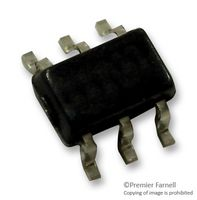
\includegraphics[width=\textwidth]{Chapter_3/ADR3425_chip.jpg}
	    \caption[]{IC}
	    \label{fig:ADR3425_chip}
	\end{subfigure}
    ~
	\begin{subfigure}[b]{.4\textwidth}
		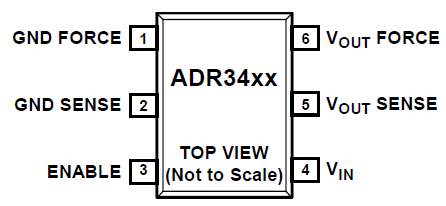
\includegraphics[width=\textwidth]{Chapter_3/ADR3425_pinout.PNG}
	    \caption[]{Pinout}
	    \label{fig:ADR3425_pinout}
	\end{subfigure}
	\rule{35em}{0.5pt}
	\caption{ADR3425 2.5V Precision Voltage Reference}
	\label{fig:ADR3425}
\end{figure}

Last component to add to the schematic, is the crystal oscillator which is required from the ADC to accurately clock the conversions. We used a simple 7.68MHz quartz crystal, following the guidance of the datasheet.

At this point we have covered all the components used in the prototype board for the electrical measurements. The complete schematic, as designed in Eagle, is given below split in -FIGURE NUMBER- and -FIGURE NUMBER- for the current path circuit and the ADC circuit respectively, because of it's large size.\\

\begin{figure}[p]
	\centering
		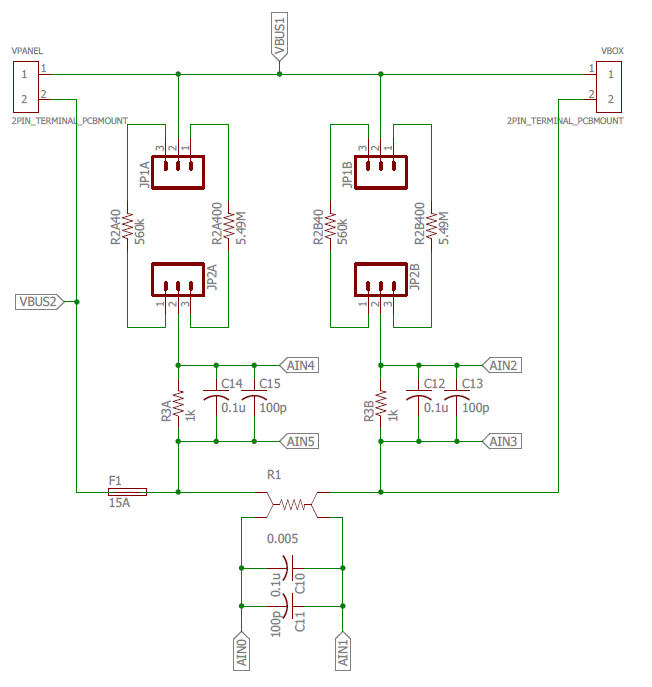
\includegraphics[width=\textwidth]{Chapter_3/PV_demo_schematic_CP.PNG}
		\rule{35em}{0.5pt}
	\caption{Current Path Schematic of demo board}
	\label{fig:PV_demo_schematic_CP}
\end{figure}

\begin{figure}[p]
	\centering
		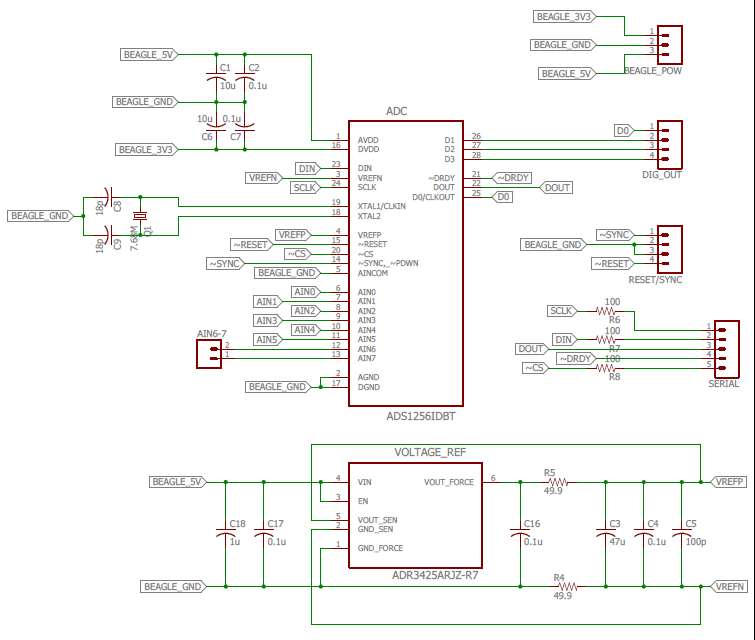
\includegraphics[width=\textwidth]{Chapter_3/PV_demo_schematic_ADC.PNG}
		\rule{35em}{0.5pt}
	\caption{ADC Schematic of demo board}
	\label{fig:PV_demo_schematic_ADC}
\end{figure}

A few points that it would be important to mention are given below:

\begin{itemize}
    \item Connectors: There are plenty of connectors and header pins used in the circuit which are displayed in the schematic as small rectangular boxes with numbered pins. We used these parts in order to connect the external wires and cables (e.g. the input and output of the PV module or the SPI bus pins) with the appropriate points in the circuit.
    \item Resistors R2A400 and R2B400: We added an extra pair of resistors to the voltage dividers in case we would like in the future to add an extra range of measured voltage instead of the default 40V. They were never used in action.
    \item Jumpers: We added jumper pins just before the voltage dividers in order to be able mainly to enable or disable each divider but additionally for choosing the desired resistance, in case of using the extra resistors mentioned above. Also, jumpers were added to the RESET and SYNC pins, to be able to change their state if needed.
    \item MISTAKE: There is a mistake in the pins RESET and SYNC of the ADC chip. Based on the datasheet and the operation we target, these two pins should be connected directly to DVDD (3.3V) but because of a design mistake they were connected to the Ground trace. This mistake was corrected in the final board.
    
\end{itemize}

After locking the schematic of the demo board, we proceed with the design of the actual board's layout. For this stage we had to take into consideration not only the dimension and footprints of each component but also the guidance of the ideal positioning for every part, based on the different datasheets. When the final layout of the board was created in Eagle, it was time to start the manufacturing process of the demo board, using a PCB university laboratory. More on the process of printing and manufacturing a PCB can be found in Appendix. The final result for the electrical measurements demo board is given in the figure -FIGURE NUMBER- as well as the complete assembled version in figure -FIGURE NUMBER-.\\

--IMAGE OF PCB LAYOUT\\

\begin{figure}[htbp]
	\centering
		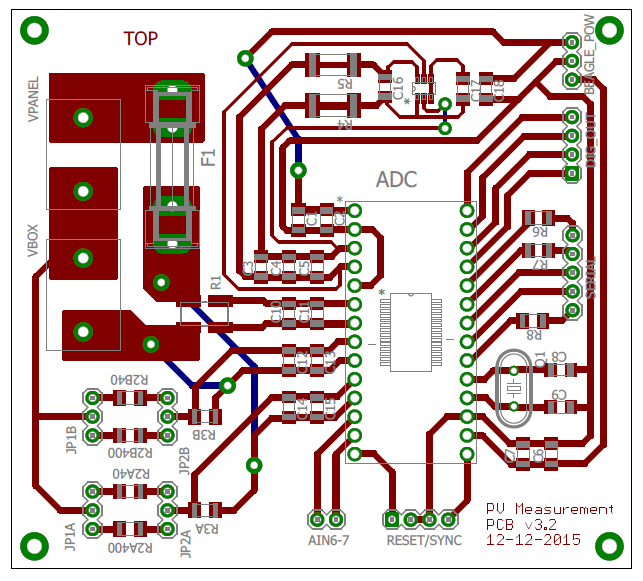
\includegraphics[width=0.6\textwidth]{Chapter_3/PV_demo_layout.PNG}
		\rule{35em}{0.5pt}
	\caption{Physical layout of demo board}
	\label{fig:PV_demo_layout}
\end{figure}

\begin{figure}[htbp]
	\centering
		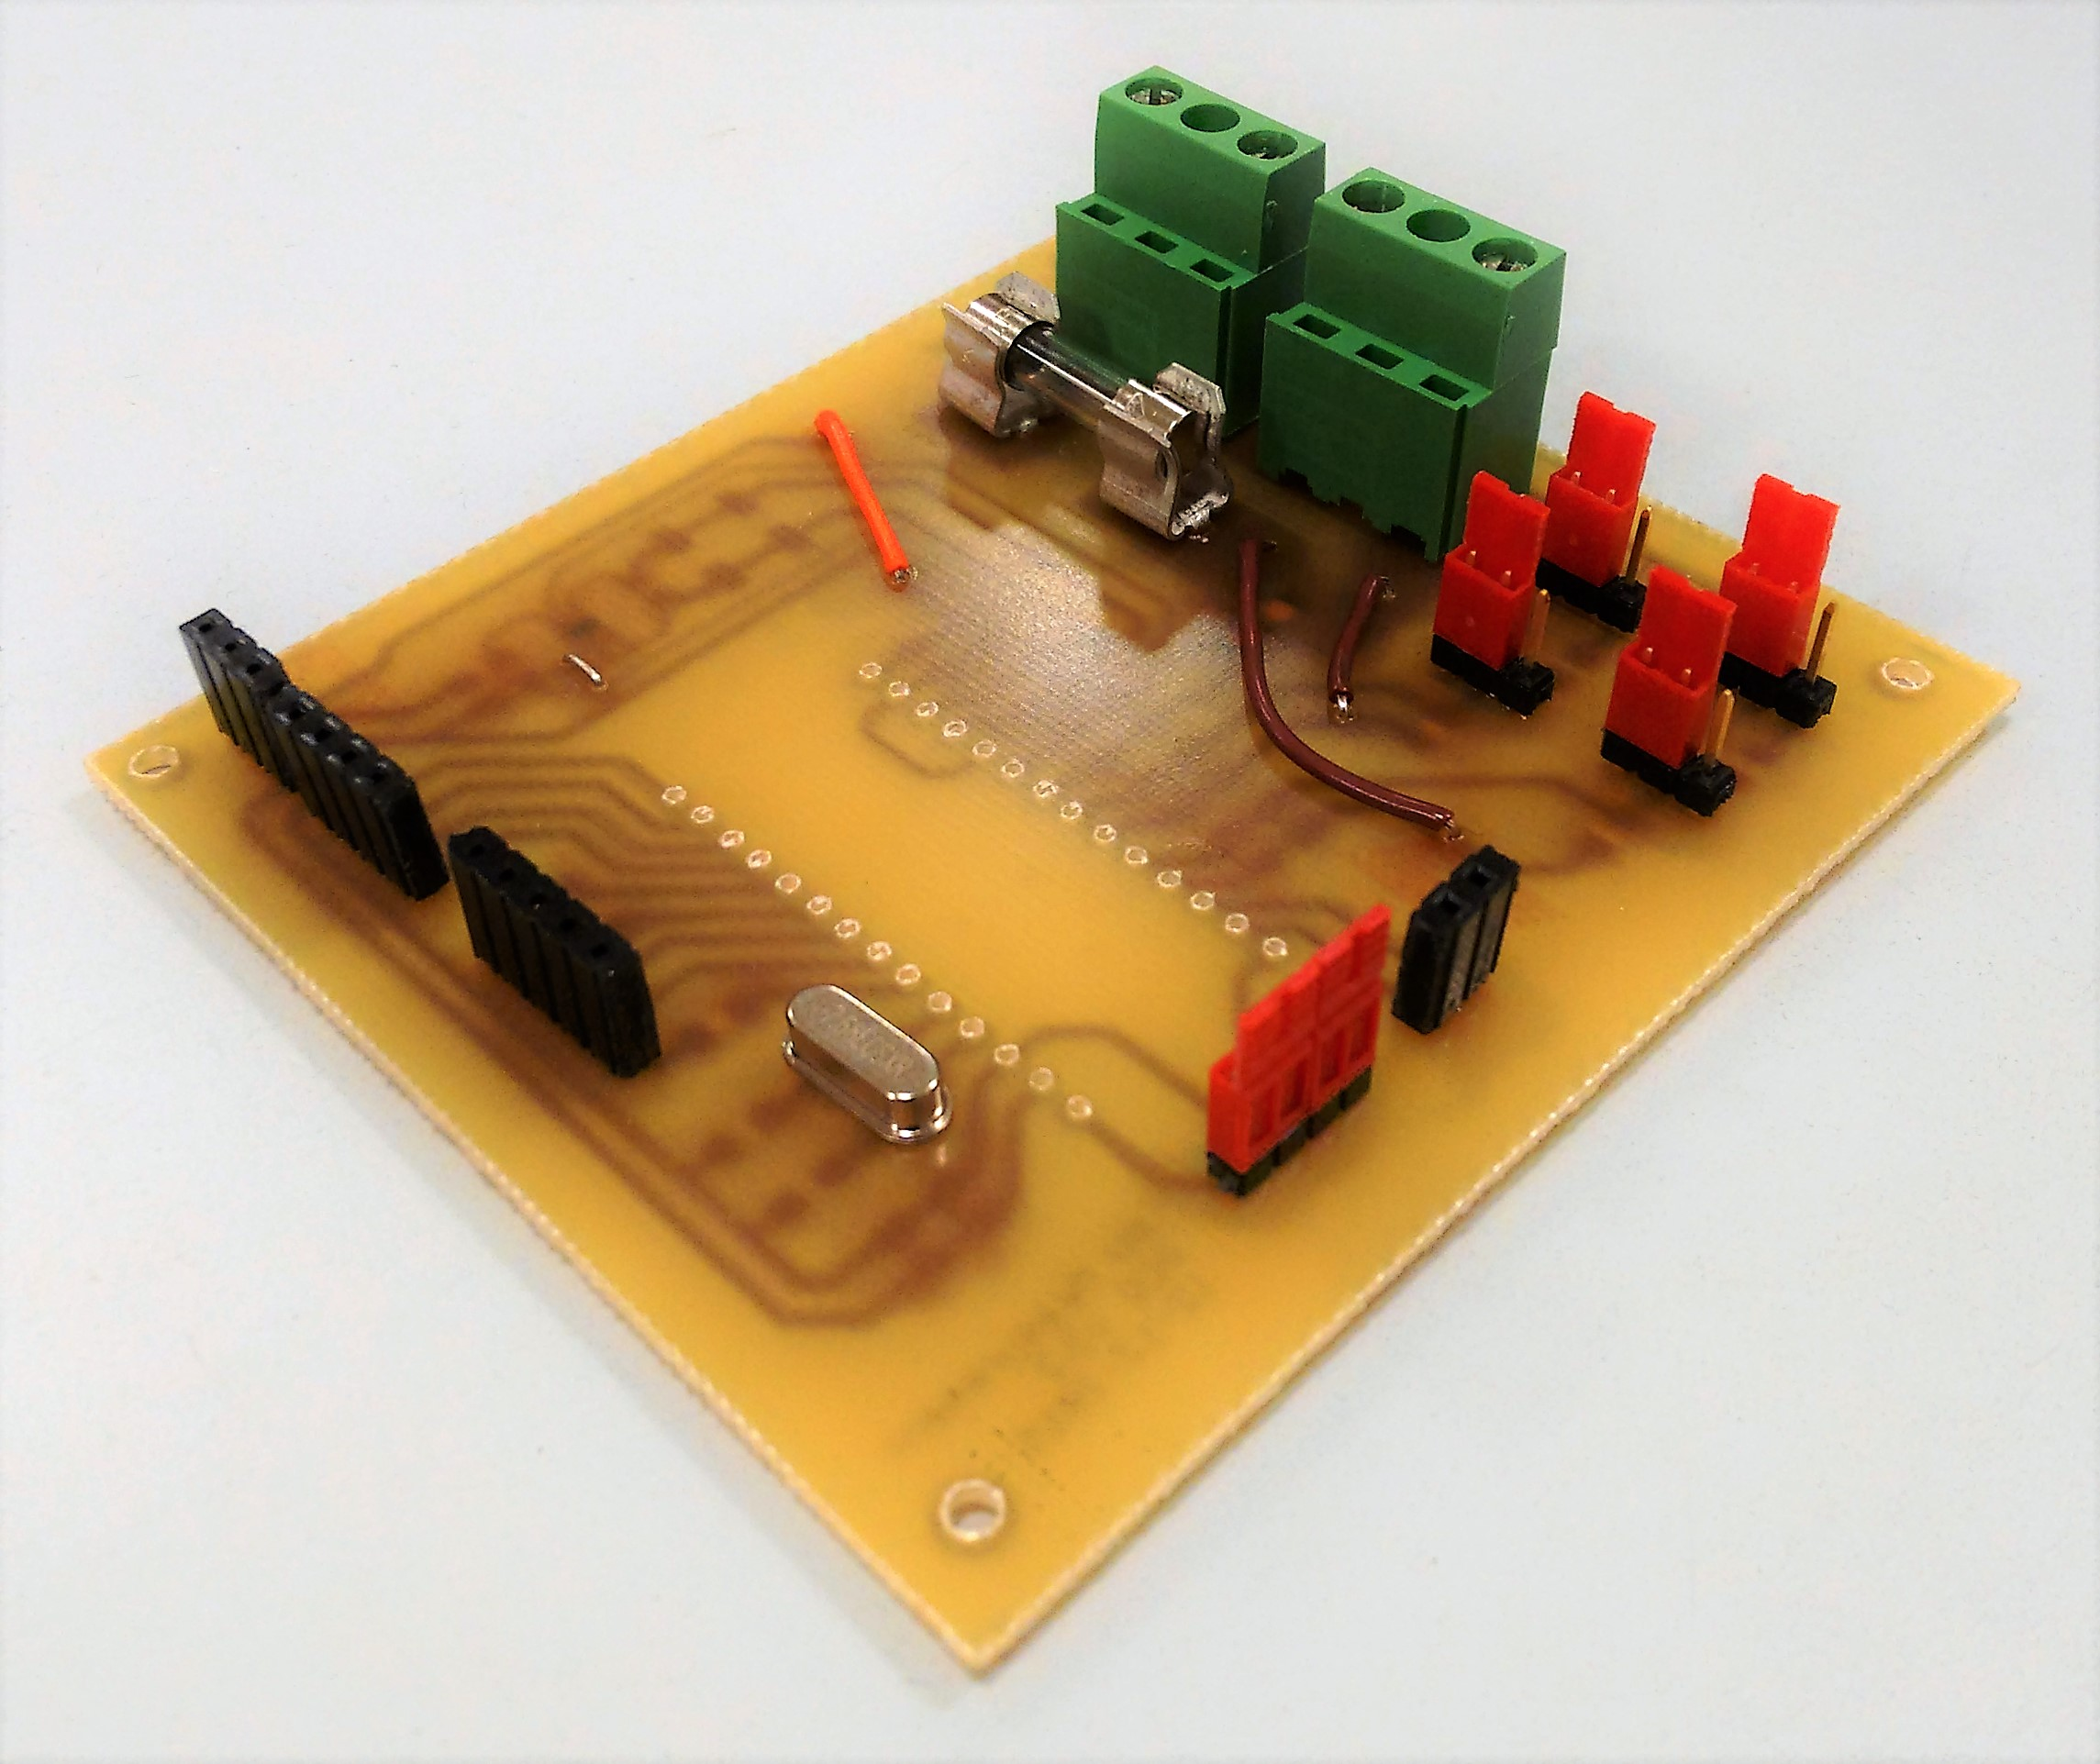
\includegraphics[width=0.6\textwidth]{Chapter_3/PV_demoPCB_assembled.jpg}
		\rule{35em}{0.5pt}
	\caption{Assembled demo board}
	\label{fig:PV_demoPCB_assembled}
\end{figure}

By observing the demo board, one can notice that:

\begin{itemize}
    \item The traces that carry the main current flow are distinctly larger in width, in comparison with any normal trace on the board, because of the high current values.
    \item The footprint of the ADC chip is not the original one, because we used an extra "breakout board", as shown in figure -FIGURE NUMBER-. This type of commercial boards are used in case of small SMD ICs' packages and consist of the actual SMD footprint of the IC and copper traces that connect the normal pads with new pins, located further away from the chip. This provides easier soldering of the SMD IC, because of the quality of the board, the soldermask etc and in the same time makes prototyping possible through common breadboard 2.54mm pin spacing.
\end{itemize} 

\begin{figure}[htbp]
	\centering
		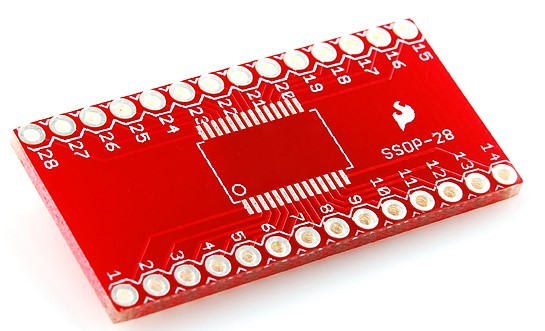
\includegraphics[width=0.5\textwidth]{Chapter_3/Sparkfun_breakout.jpg}
		\rule{35em}{0.5pt}
	\caption{Sparkfun Breakout board for the ADS1256}
	\label{fig:Sparkfun_breakout}
\end{figure}

As we discussed earlier, there is no microcontroller chip on the board, as we will use the Arduino Uno board for the control and acquisition of the measured data. So at this point, after the assembly and soldering of the board, we had to start testing the new demo board and check if the ADC can provide the measurements as requested. The steps of this prototyping and testing stage are given below:

\paragraph{1. Wiring to Arduino\\}
For this step we used simple breadboard cables to create all necessary connections. The couples of pins from the measurement demo board and the corresponding ones on the Arduino board are given in the table -TABLE NUMBER- below.

\begin{center}
\begin{tabular}{ l l l } 
 Measurement board & Arduino Uno Pin & Description \\ \hline
 5V & 5V & Main power supply voltage of 5V \\ 
 3.3V & 3.3V & Digital power supply voltage \\
 SCLK & SCK(13) & Clock line for SPI communication\\
 DIN & MOSI(11) & MOSI signal for SPI communication\\
 DOUT & MISO(12) & MISO signal for SPI communication\\
 DRDY & INT(2) & Interrupt pin, used as "data ready" flag\\
 CS & I/O(7) & Simple chip select pin for ADC enabling\\
\end{tabular}
\end{center}

\paragraph{2. Register configuration\\}
First important point to mention is that during the development of the code we found and used an Arduino library, written by the Jonathan Graesser, for the ADC chip ADS1256. This library really pushed the development process further and saved us a huge amount of time, which we were able to spent on testing and further designing.

The code development started with the basic objective, the simple voltage sensing. This requires firstly to set the appropriate registers of the ADS1256 in order to configure the setting parameters of the conversion such as which input channel is used, the programmable gain, the sampling frequency etc. More specific, the values of the registers that we set at this point of the programming are given in the table below:

\begin{center}
\begin{tabular}{ l l l } 
 Register & Value & Description \\ \hline
 Name & XXX & mpla mpla mpla
\end{tabular}
\end{center}

\paragraph{3. Simple voltage measurement\\}
After setting the above register configuration, we are able to make the first actual voltage measurement. At this point the value we get back from the Arduino is not mapped, so using the datasheet we have to find the mapping function to get closer to the real voltage value that is measured. This draft calibration stage is carried out using a laboratory DC voltage power supply, a multimeter and the values we get from the analog to digital conversion. The correction parameters can be calculated through a simple Microsoft excel spreadsheet, combining the useful mapping information from the ADS1256's datasheet and the measured values from logging of the DC power supply voltage points.

\paragraph{4. Complete electrical measurement (V1, V2, I)\\}
Next step is the addition of two more measurements, using the two more input channels of the ADC. This is possible by altering the MUX register and choosing the appropriate pair of input pins for each measurement differential input. In order to make the testing easier, a simple Processing script was developed at this point visualising all three measurements to a screen of a laptop connected to the monitoring Arduino board.

The same technique is used to map all three measured values this time, the two voltages from the voltage dividers as well as the current from the voltage drop across the shunt resistor. The final result at that point is a prototype setup, able to monitor both voltage and current at the input of the board with efficient accuracy but with no time respect at all, meaning no time keeping has been carried out yet.

\subsubsection{Temperature sensing}
Having sorted out the main philosophy and code of the electrical measurements, we can focus also on the temperature sensing and timing of the measurements. Concerning the temperature, as discussed earlier, we use the digital temperature sensor DS18B20 which communicates with the microcontroller through the 1-Wire bus protocol. The initial prototyping started with a single sensor and an Arduino Uno board running code only relevant with the temperature measurement. 

During this stage, we defined the desired configuration for the sensing through a range of registers, similar with the ADC chip. In particular we chose the following settings:

\begin{center}
\begin{tabular}{ l l l } 
 Register & Value & Description \\ \hline
 Name & XXX & mpla mpla mpla
\end{tabular}
\end{center}

After this initial test set-up, four more sensors were added to the circuit using a common breadboard. The code was updated accordingly and after a few failed attempts, we managed to confirm the capability of multiple sensors to operate on the same bus. Next goal was to re-enable the electrical measurements which we had skipped for the first temperature sensing experiments. Both the physical circuit and the code were modified resulting the setup shown in the figure -FIGURE NUMBER-, in which one can notice the demo board, the Arduino and five DS18B20 sensors. One more thing to mention here is the addition of a $4.7k\Omega$ pull-up resistor to the data bus of the 1-Wire bus, as stated in the protocol documentation.\\

\begin{figure}[htbp]
	\centering
		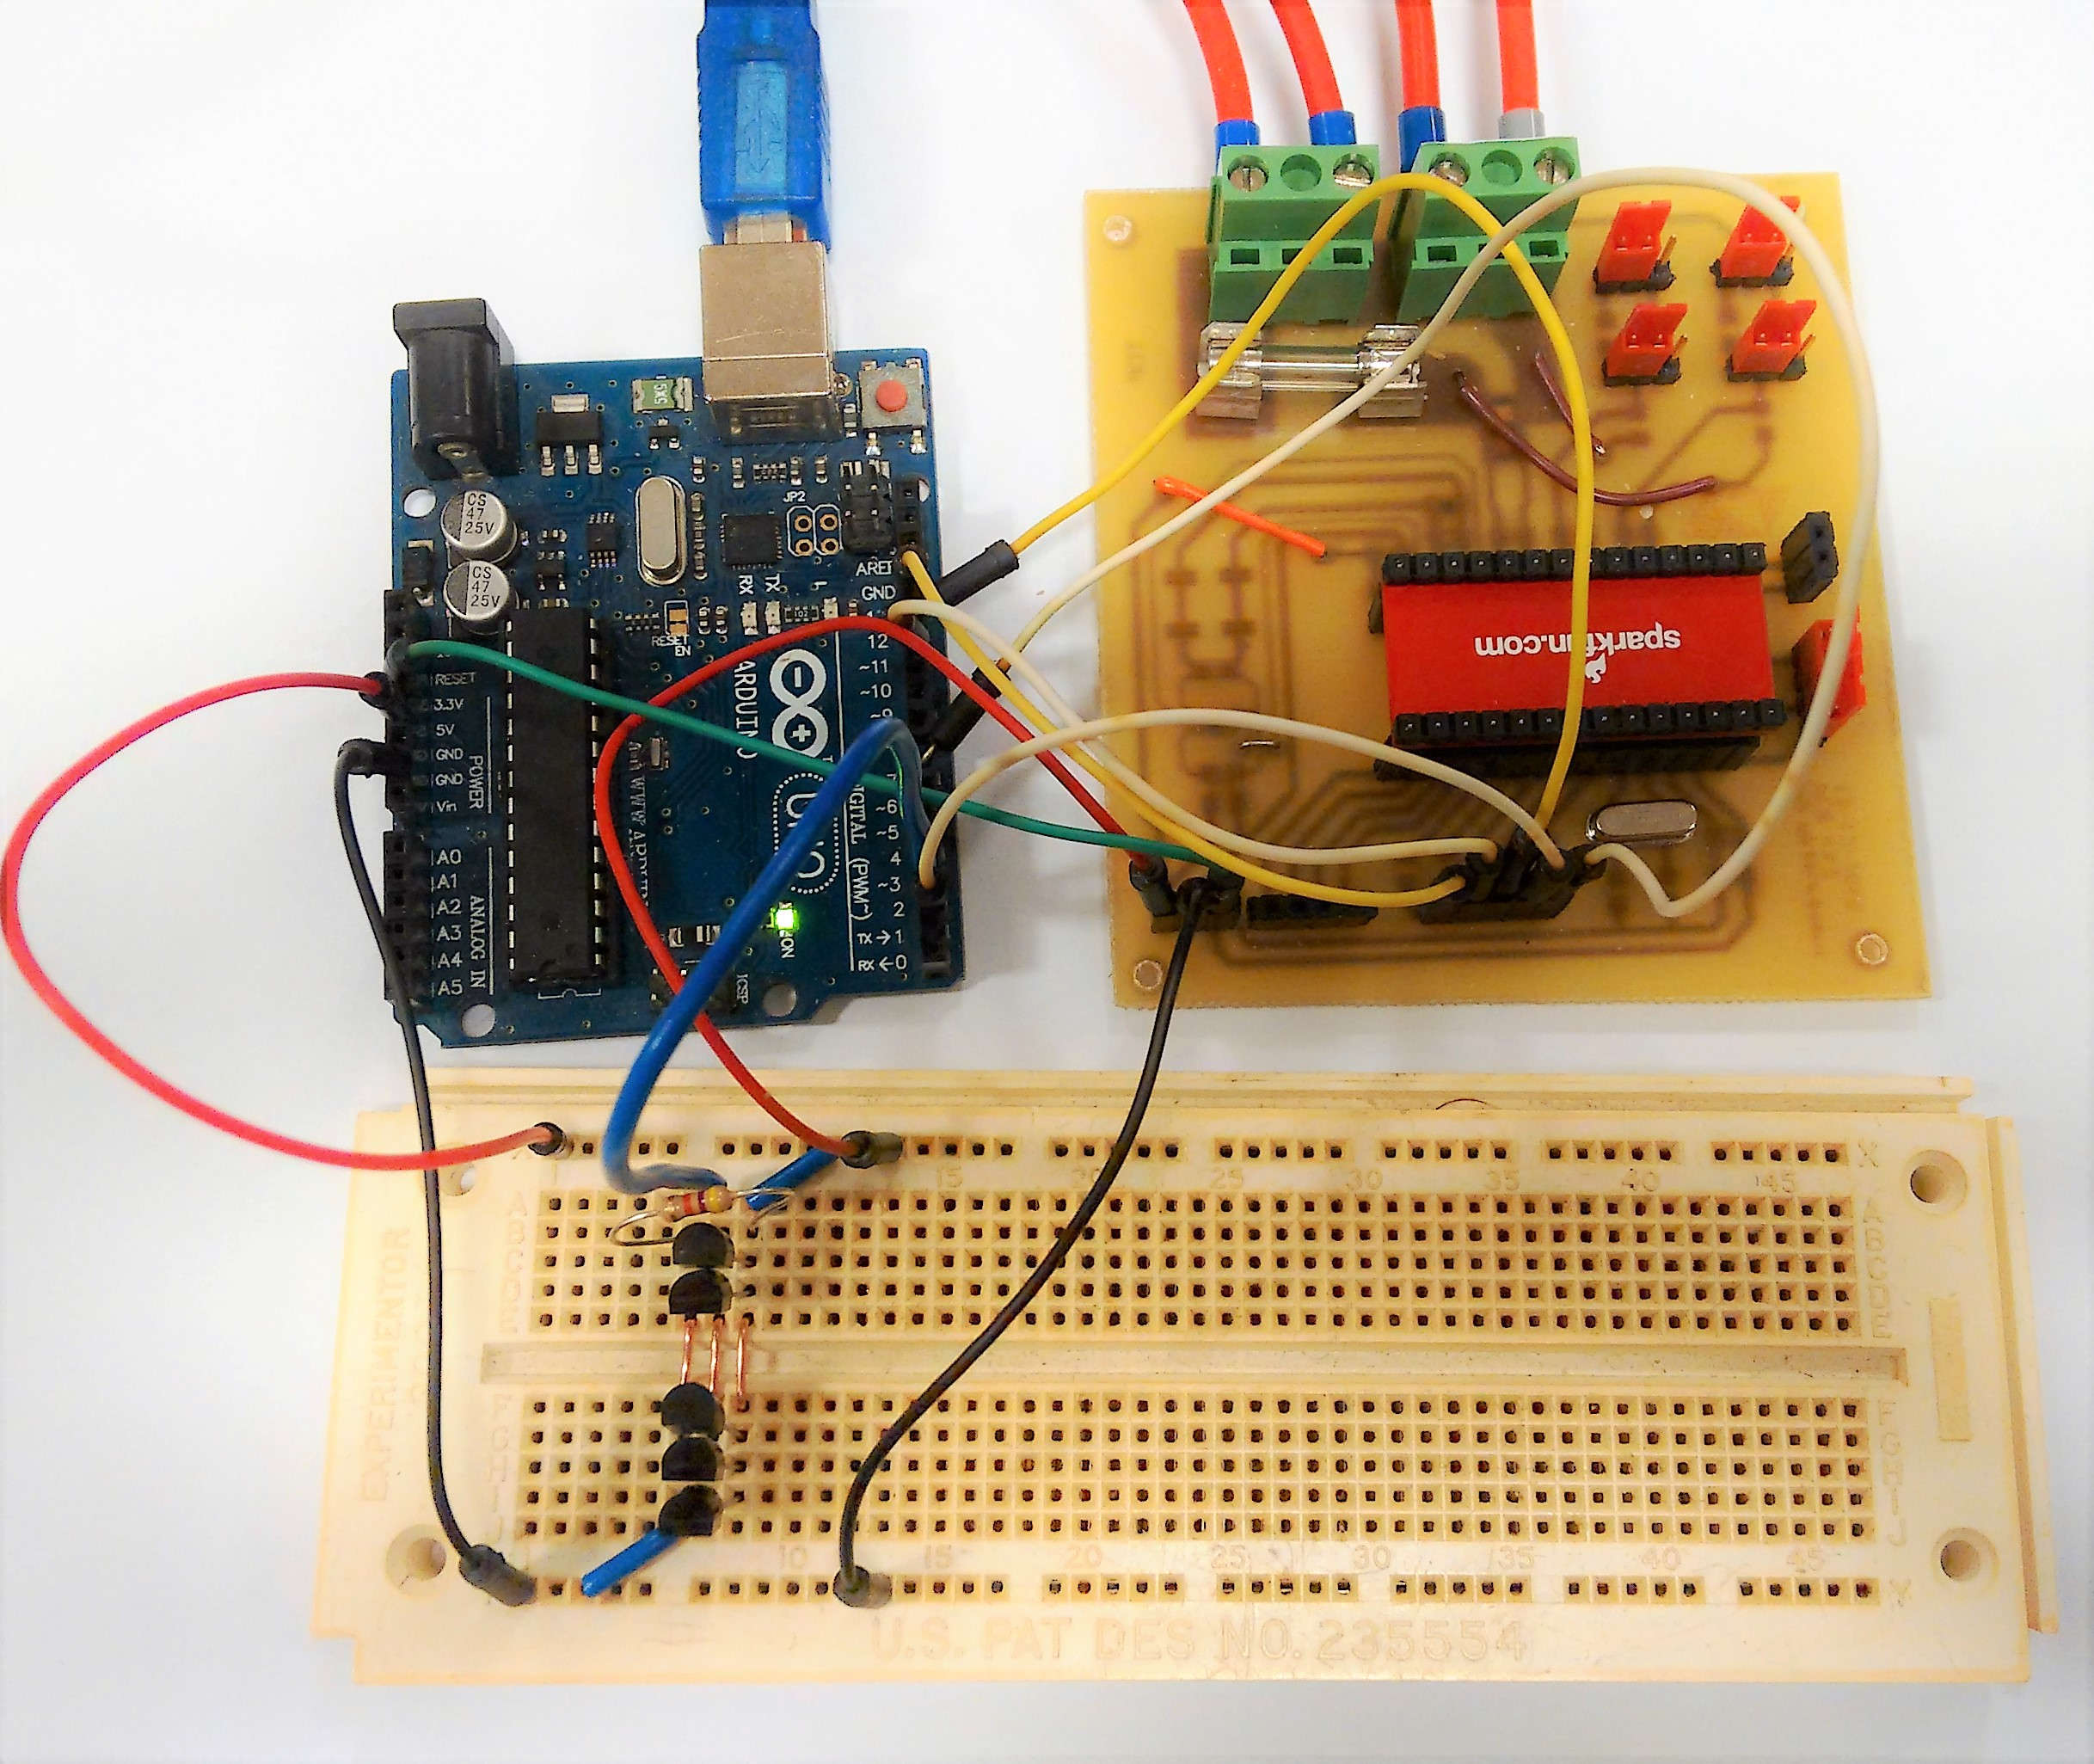
\includegraphics[width=0.9\textwidth]{Chapter_3/prototype_Elec5Temp.jpg}
		\rule{35em}{0.5pt}
	\caption{Initial prototype setup (Arduino, demo PCB, 5xDS18B20)}
	\label{fig:Sparkfun_breakout}
\end{figure}

With the previous setup it was possible to experiment with the code and find the most suitable configuration, in terms of register values, for both the ADS1256 converter and the DS18B20 sensors. Adding the 15 more temperature sensors to the breadboard, in order to achieve the initial project's goal  of 20 temperature points in total was rather simple, as we had to follow the same process with the addition of the first 5 sensors. The only question that may arises at this point is what is the required time to get all the measurements, including both the electrical values and all 20 temperatures. To answer this question we need to proceed to the next subject, which is timing.

\subsubsection{Measurement clock}
As we described in the beginning of this chapter, the solution for all timing and clocking tasks in the board is the use of a RTC and specifically, the IC we chose is the DS3234. This device comes in a compact 20-SO SMD package, which makes the prototyping with the IC nearly impossible without a proper board. For this reason, we used a specific board, which belongs to a wide category of PCBs called modules. These boards usually facilitate a core component, in this case the RTC chip, and accompany the IC with all necessary circuitry and parts such as capacitors, resistors, voltage regulators, buttons, LEDs, connectors etc. In this way it is tremendously easier to prototype, as connections are more accessible even on a common breadboard. The DS3234 RTC module is commercially produced by SparkFun and is shown in the figure -FIGURE NUMBER-.\\


\begin{figure}[htbp]
	\centering
		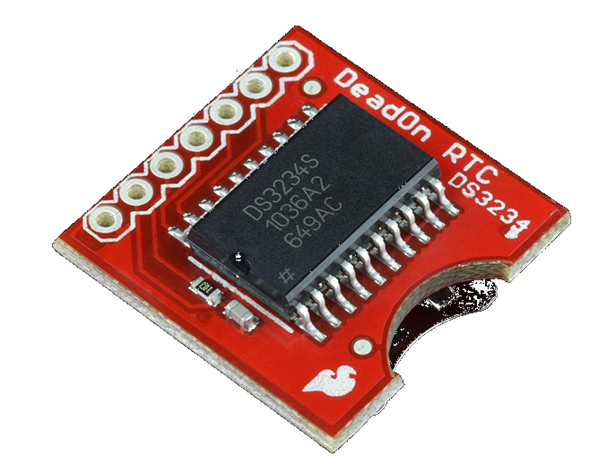
\includegraphics[width=0.4\textwidth]{Chapter_3/Sparkfun_RTC.PNG}
		\rule{35em}{0.5pt}
	\caption{Sparkfun RTC DS3234 module}
	\label{fig:Sparkfun_RTC}
\end{figure}

With the convenience of this board, we can add the RTC to the existing setup and proceed with the clocking implementation. The first experiments were made only with the combination of the Arduino Uno and the RTC module to keep the understanding process simple. After the first successful experiments, we included the module to the measuring setup, once again using the breadboard. The physical setup is shown in the figure -FIGURE NUMBER-.\\

--IMAGE OF SETUP WITH ARDUINO, DEMO PCB, DS18B20 AND RTC \\

The code development process is very similar with the cases of the ADC and the temperature sensors. Using the appropriate library, we start by setting the values of a few registers hence configuring the way the RTC operates. Next, we are able to set the current time as well as get the timestamp in a simple data format, which we can include in the measured data. One important step during the software development for the RTC is the precise 1Hz clock signal generation and more specific the way the Arduino handles it. In particular, a simple change in a register of the DS3234 is enough to enable the 1Hz square wave pulse output in the corresponding pin of the IC. But how can we use this pulse for the timing of the measurements in the Arduino side? The solution is a common timing technique used in several microcontroller scenarios, called interrupts.

This technique uses either an internal timer or, in our case, an external signal as a trigger of an event. When this trigger is activated, the microcontroller runs a specific part of code especially written as an interrupt routine. Having this method in mind, we used the 1Hz pulse of the RTC to act as the trigger of the interrupt and started developing the software. One problem we faced was that the measurement of all temperatures was taking too much time resulting a total measuring time, for all desired data, more than one second. This issue was solved by modifying the way the microcontroller handles the temperature sensor and specific the safety time it has to wait from the temperature request until the acquisition of the result. The way to overcome that was to firstly request the temperature from all 20 sensors and after that, instead of holding the microcontroller inactive to wait the result, use it to get the electrical measurements and then come back to the temperature results.

To simply describe the order of the tasks that the microcontroller executes, we collected them in the following list:

\begin{enumerate}
    \item Request the temperature measurements from all 20 sensors and continue the execution
    \item Get the electrical measurements by changing the ADC input channel
    \item Get the temperature results from the sensors
    \item Get the current moment from the RTC
    \item Hold the microcontroller inactive until the interrupt (1Hz pulse) happens
\end{enumerate}

The above tasks are being executed in this order over and over again as an endless loop. One important point that we need to highlight is the last "waiting for the interrupt" process. Programming using this method can guarantee that the code will start execution precisely every one second and as a consequence the measurements will take place with the same desired frequency of 1Hz. Last experiment we did with this setup is to get the amount of total run time for the measurements. The results show that the microcontroller is able to acquire every value needs to be measured, including all 20 temperatures and the timestamp, in around 600ms resulting around 400ms of free time for extra functions we will discuss in the next paragraphs.


\subsubsection{Control Device simulation}
So far we have managed to assemble a functional prototype setup, consisting of the following components:

\begin{itemize}
    \item Arduino Uno board
    \item Demo measurement board
    \item 20 temperature sensors (with the necessary pull-up resistor)
    \item RTC module
\end{itemize}

This means that we created the core of the measuring system. But in order to be confident about the design we need to test the current prototype more and explore its capabilities and potential malfunctions. Consequently we need a second system as the control device, whose main role will be to request the measured data from the measuring system and store them in some kind of storage. As we have not developed this system yet, we can use a similar prototype setup to simulate its main function of requesting the data packets from the measuring part. In the boundaries of prototyping, we used a second Arduino Uno board to play this role of the "control device", featuring only the main task of requesting the data.

There are a few different approaches to achieve communication between digital systems like the ones we have described so far including serial communication, I$^2$C etc. The protocol we chose for the communication between the two parts of the system is the I$^2$C because firstly it has more than sufficient data rate but mainly because it uses only the two available I$^2$C pins for the bus. This is really important because the SPI pins of the atmega, in the measuring part, are already used for the communication with the ADC and the RTC. Although it is possible and even common to connect multiple devices to a single SPI bus, there is an important factor to take into consideration. One device should be either master or client in this type of communication, which creates a problem in the case of the atmega in the measuring part. More specific, this microcontroller has the role of master in the communication with the ADC and RTC but should be client in the communication with the control device. Therefore using I$^2$C instead of SPI is the most promising solution.

The connections between the two parts are given below:

\begin{center}
\begin{tabular}{ c c p{5cm} } 
 Measuring Arduino & Control Arduino & Description \\
 (Client) & (Master) & \\\hline
 5V & 5V & Power supply line \\
 GND & GND & Ground line \\
 SDA(A4) & SDA(A4) & Data line of I$^2$C bus \\
 SCL(A5) & SCL(A5) & Clock line of I$^2$C bus \\
 DATA-READY(7) & INT(3) & Interrupt line, activated when the data packet is ready \\
\end{tabular}
\end{center}

The code on the second Arduino Uno is developed in the direction of only simulating the control device. In particular it is waiting for the data packet to be created in the measuring side and when this happens, the interrupt pin (3) get activated resulting the stop of microcontroller's hold. After this waiting time, the Arduino in the control side request the measured data from from the measuring Arduino.

At this point we have only discussed the tasks of the Arduino at the control side, but how the measuring microcontroller handles the communication and data transfer? For this question we have to firstly describe, with more details, what is happening on the measuring Arduino. As we discussed in the previous section, the measuring microcontroller is able to get all measurements in the first 600ms and then wait the rest 400 ms, until the next 1Hz pulse is activated. We can use this "free time"  for the construction of the data packet and later on its  transmission to the control device. Because the transferred data in the I$^2$C communication have a specific maximum length of 32 bytes, we need to split the measured values in 6 packets each one of them consisting of different measurements, as noted in the table -TABLE NUMBER-.

\begin{center}
\begin{tabular}{ c l } 
 $\#$ & Data \\ \hline
 1 &  Timestamp and Current\\
 2 &  Two Voltages and Power\\
 3 &  Temperatures 1-5\\
 4 &  Temperatures 6-10\\
 5 &  Temperatures 11-15\\
 6 &  Temperatures 16-20\\
\end{tabular}
\end{center}

After the construction of these six data packets, the measuring microcontroller is ready to send the data to the control side, therefore it activates the "data ready" flag pin which activates the corresponding interrupt. The control device request one data packet each time, by sending its number to the measuring microcontroller. The last one read the requested packet's number and send it to the control device.

Summing up the above discussed subjects, at this point we have created a functional prototype of the measuring system as well as a simulating circuit for the control side. This combination of prototype setups gives us the opportunity to test the measuring system as a whole and further develop the firmware. As a result we can finalize the circuitry and proceed to the last steps before the final design of the measurement PCB.

\subsubsection{Isolation board}
The only goal not achieved yet with the current prototype setup is the isolation layer between the two parts of the system. As we have described earlier, we have concluded which ICs will be used for the isolation of both the power supply and the communication signals. So, the only missing part is the actual design of the isolation stage. For this reason we decided to create a new demo PCB, specifically designed to test the isolation setup that we have in mind.

This board facilitates the ADuM5000 isolated DC-to-DC converter as well as the MAX14850 six-channel digital isolator. Moreover, there are added a few more parts necessary for the operation of the two ICs such as decoupling capacitors, along with the appropriate pin headers for the external connections during prototyping. Four pull-up resistors are also necessary for the I$^2$C bus lines, as mentioned in the MAX14850's datasheet. The final schematic of this board is really simple and is shown in the figure -FIGURE NUMBER-. Simply described, the board takes the signals from the pin header in the "non-isolated" side and pass them through the appropriate isolation IC which in the end feeds them to the header pin in the "isolated" side.\\


\begin{figure}[htbp]
	\centering
		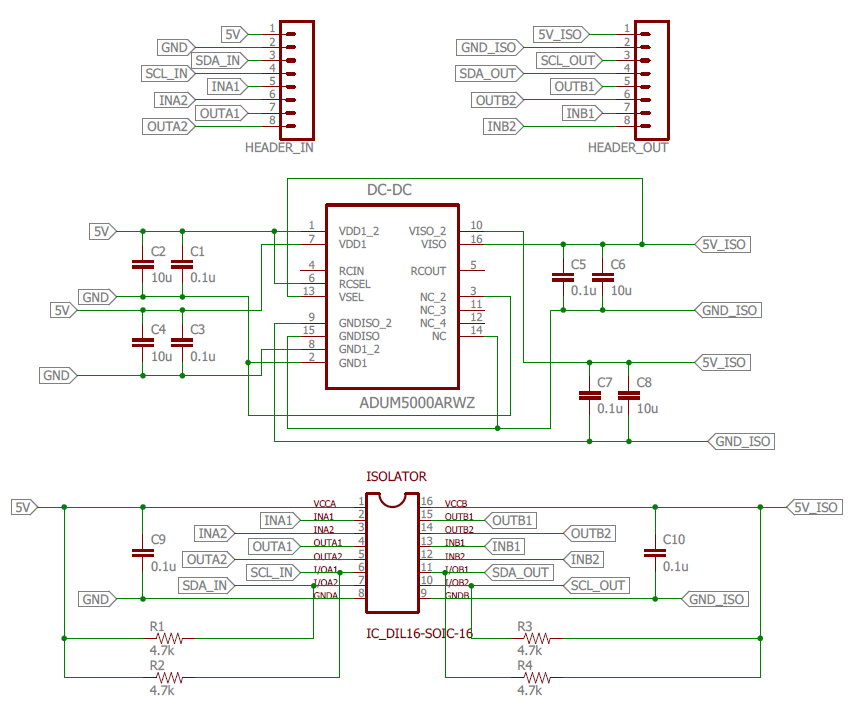
\includegraphics[width=0.9\textwidth]{Chapter_3/ISO_demo_schematic.PNG}
		\rule{35em}{0.5pt}
	\caption{Isolation demo board schematic}
	\label{fig:ISO_demo_schematic}
\end{figure}

The manufacturing of the board was carried out with exactly the same techniques as the demo PCB for the electrical measurements. We used the university's PCB laboratory and finally printed the demo Isolation PCB, as shown in the figure -FIGURE NUMBER-. More information about the PCB fabrication in the laboratory is given in the Appendix.\\

\begin{figure}[htbp]
	\centering
		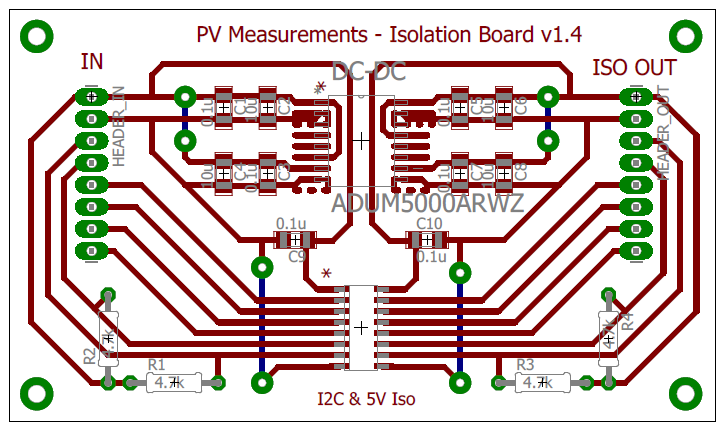
\includegraphics[width=0.8\textwidth]{Chapter_3/ISO_demo_layout.PNG}
		\rule{35em}{0.5pt}
	\caption{Isolation demo board layout}
	\label{fig:ISO_demo_layo}
\end{figure}

HERE MAYBE ADD THE MODIFICATION I DID DURING PROTOTYPING???
SOMETHING WAS WRONG BUT I DON'T REMEMBER, I HAVE TO CHECK THE BOARD AT HOME!!


\subsection{Final Design}
After many hours of designing and testing the prototype boards, fixing minor or sometimes major problems and issues in both hardware and software it is time to make the next step. This stage is the design of the final PCB that will be included in the final device in order to carry out all the measurements and transfer the acquired data to the control part. In the following sections we will discuss all the changes and improvements we had to make in order to pass from the prototyping area to the final design, we will present the physical layout of the final PCB and lastly describe the process of assembling and testing the new board.


\subsubsection{Schematic}
Starting point of this new design is the updated schematic of the measuring circuit. The PV Measurements PCB is combining all previous boards' functions and therefore it's schematic consists mostly of previous boards with a few addition and changes. In particular, we kept almost the same circuits for the electrical measurements, the analog to digital conversion, the isolation and the 2.5V voltage reference. On the other hand, completely new designs were necessary for the real time clock circuitry, the 3.3V voltage regulation, the microcontroller and of course the board's external connections.

To sum up all information mentioned in previous sections, the new PCB should be able to carry out the following tasks:

\begin{itemize}
    \item Precisely measure the current and voltage of the PV module's output
    \item Sense up to 20 temperature points
    \item Clock the above measurements, accurately once every one second
    \item Isolate the output of the board from the rest circuit
    \item Transfer the logged data to the connected control device through I$^2$C
\end{itemize}

 The circuit we come up with is shown as Eagle schematic below, but because of its large size it is split in three different sections. More specific the electrical measurements and ADC circuits are shown in figure -FIGURE NUMBER-, the isolation layer, the 2.5V voltage reference and the 3.3V regulation circuits are shown in figure -FIGURE NUMBER- and lastly in the figure -FIGURE NUMBER- are presented the circuit of the microcontroller, the RTC and all board's external connections. At this point, it is important to highlight that all these four parts of the circuit belong to the same big schematic design, and one can notice the connection points between them using the reference labels, marked in gray.\\
 
 \begin{figure}[htbp]
	\centering
		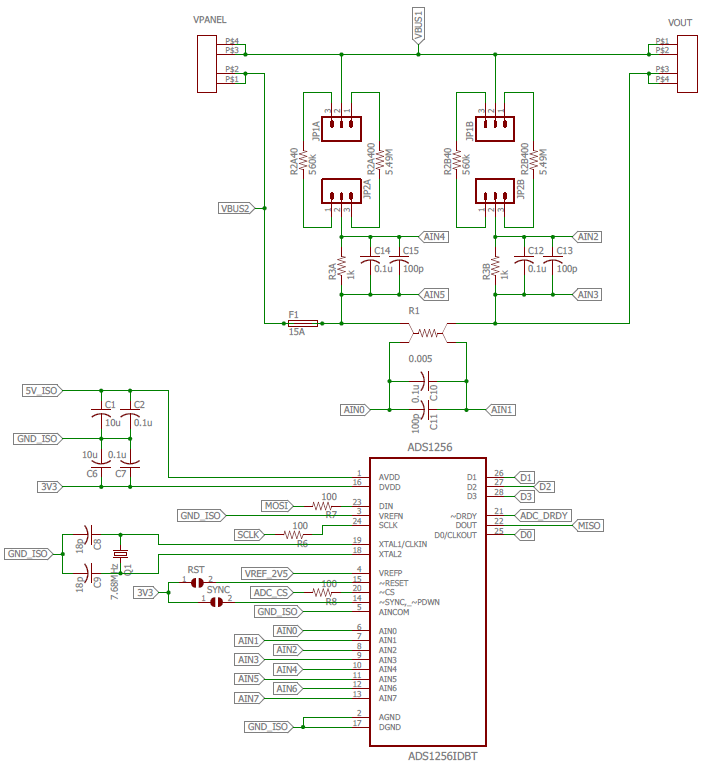
\includegraphics[width=\textwidth]{Chapter_3/PV_MeasPCB_CP_ADC.PNG}
		\rule{35em}{0.5pt}
	\caption{Schematic of electrical measurement and ADC circuitry}
	\label{fig:PV_MeasPCB_CP_ADC}
\end{figure}
 
 HERE mention the changes from the first demo board, such as RESET and SYNC pins etc\\
 
\begin{figure}[htbp]
	\centering
		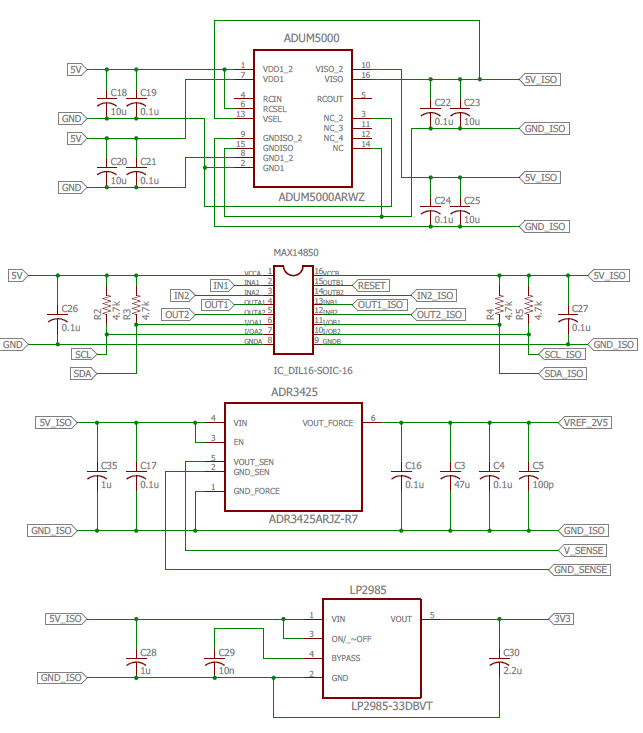
\includegraphics[width=\textwidth]{Chapter_3/PV_MeasPCB_ISO_2V5_3V3.PNG}
		\rule{35em}{0.5pt}
	\caption{Schematic of isolation, 2.5V voltage reference and 3.3V regulation circuitry}
	\label{fig:PV_MeasPCB_ISO_2V5_3V3}
\end{figure}
 
 HERE mention the changes from the iso demo board, and the describe briefly the design of the 3.3V regulation\\
 
\begin{figure}[htbp]
	\centering
		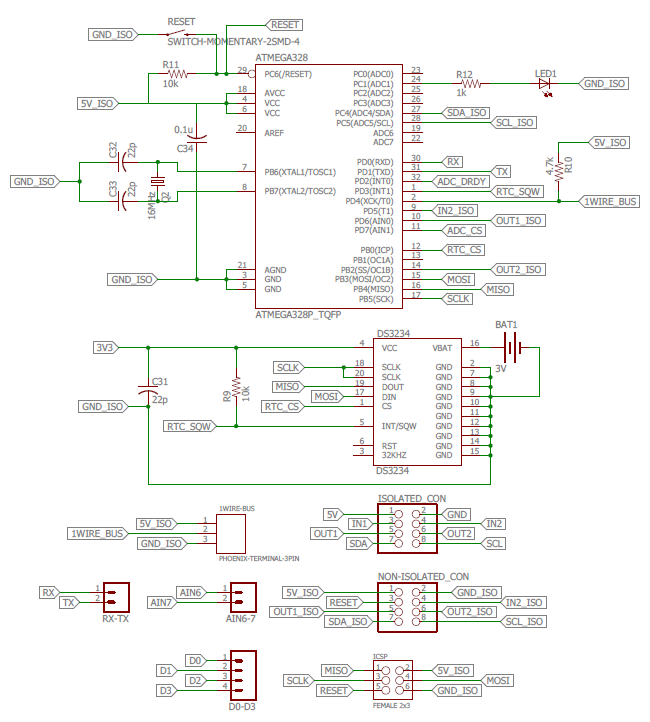
\includegraphics[width=\textwidth]{Chapter_3/PV_MeasPCB_ARD_RTC_CONNEC.PNG}
		\rule{35em}{0.5pt}
	\caption{Schematic of microcontroller, real time clock circuitry and external connections}
	\label{fig:PV_MeasPCB_ARD_RTC_CONNEC}
\end{figure}
 
 HERE describe the circuit of the atmega, the real time clock and all the connections
 also mention: RX-TX pins for debugging, LED indicator, Reset button
 
 Last but not least, it is important to describe the main function of each connector of the board, including the header pins, the jumpers etc. In the table -TABLE NUMBER- below we have collected all these connections points on the board with a brief description.\\
 
 --TABLE OF CONNECTORS\\
 
\subsubsection{Layout}
Once the schematic is drawn with all the parts and connectors wired, we can proceed to the design of the physical layout that the PCB will have. At this stage, there are plenty of interesting points that the design philosophy matters such as the components positioning or the width of the traces and the distance between them. For this reason we will present the final PCB's layout and after that focus on individual parts of the board in order to describe in depth these crucial design details. The physical layout of the PV Measurement PCV, at version 2.7, is shown in the figure -FIGURE NUMBER- as realistic rendering.\\


\begin{figure}[htbp]
	\centering
	\begin{subfigure}[b]{.45\textwidth}
		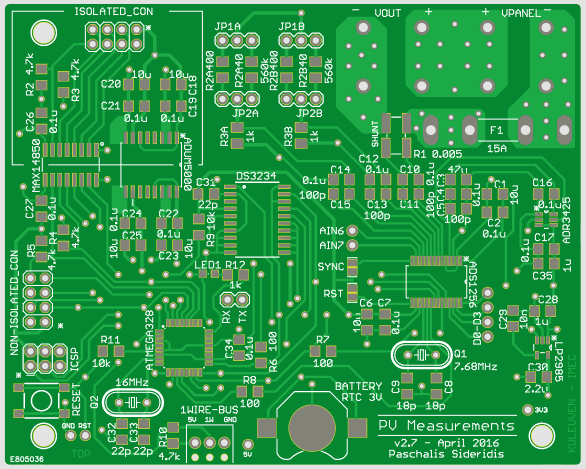
\includegraphics[width=\textwidth]{Chapter_3/PV_MeasurementPCB_top.PNG}
	    \caption[]{Top view}
	    \label{fig:PV_MeasurementPCB_top}
	\end{subfigure}
    ~
	\begin{subfigure}[b]{.45\textwidth}
		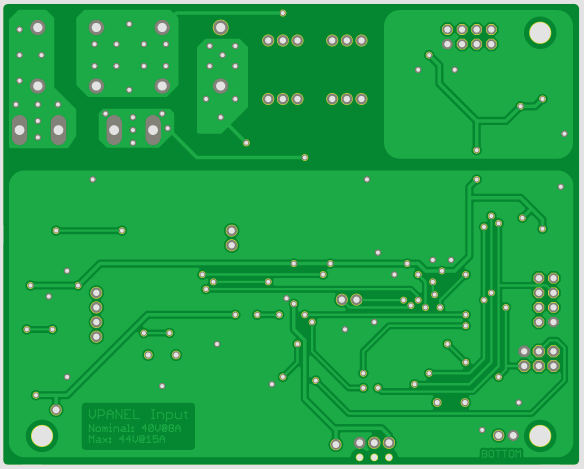
\includegraphics[width=\textwidth]{Chapter_3/PV_MeasurementPCB_bottom.PNG}
	    \caption[]{Bottom view}
	    \label{fig:PV_MeasurementPCB_bottom}
	\end{subfigure}
	\rule{35em}{0.5pt}
	\caption{PV Measurements PCB realistic rendering}
	\label{fig:PV_MeasurementPCB_render}
\end{figure}

The first part of the board that requires special mention is the circuit in which the main current flows. It is shown in figure -FIGURE NUMBER- as represented in Eagle board environment.\\


\begin{figure}[htbp]
	\centering
		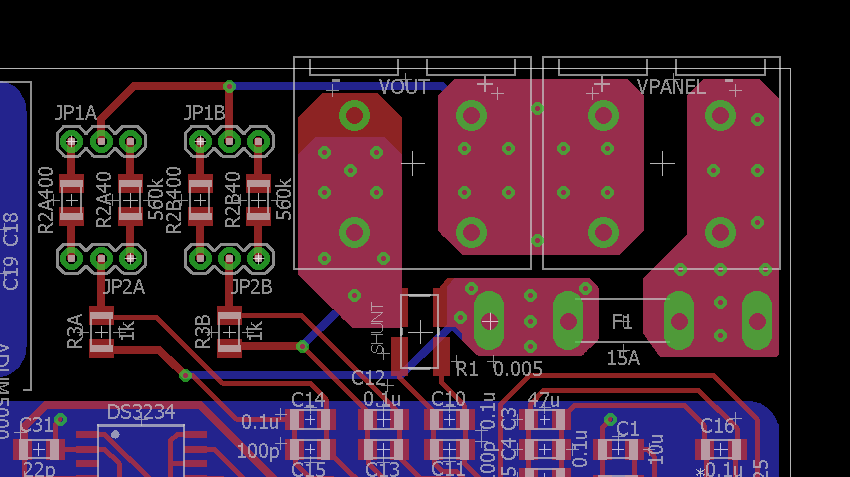
\includegraphics[width=0.7\textwidth]{Chapter_3/PV_MeasPCB_ZOOM_CP.PNG}
		\rule{35em}{0.5pt}
	\caption{Current path as shown in Eagle board environment}
	\label{fig:PV_MeasPCB_ZOOM_CP}
\end{figure}

By observing the board's layout, one can easily notice the very big size of the copper traces used for this circuit. Also, an interesting design point is the multiple vias that connect the top and bottom layers, which have almost identical trace shape, inside the current path. The reason behind both of these design choices is the high values of current that flow through the copper traces. Because of this high current values it is important to increase the conductive material of the path, resulting less resistance and consequently less output influence, temperature losses etc.

The shape of the copper traces is not designed like so for no reason either. As you may notice, all corners of the wide copper traces are broken into radius to decrease the chance of short between the different parts of the circuit, carrying high current. For the same reason we kept these traces away from each other as well as from the main ground plane of the board.

Next part of the layout that we will zoom in is the area around the ADC chip, as shown in the figure -FIGURE NUMBER-.\\

--CORRECTIONS HEREEEEEE!!! IMAGE OF ADC IN EAGLE with arrows to the vsense lines of the voltage reference\\
\begin{figure}[htbp]
	\centering
		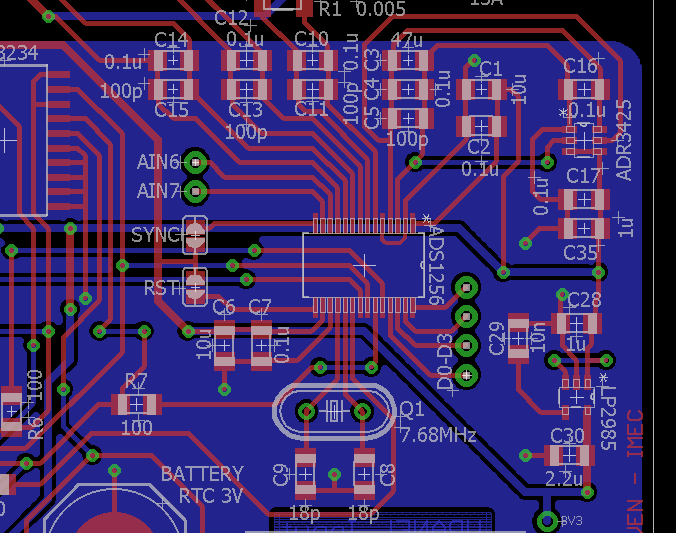
\includegraphics[width=0.7\textwidth]{Chapter_3/PV_MeasPCB_ZOOM_ADC.PNG}
		\rule{35em}{0.5pt}
	\caption{ADC circuitry layout as shown in Eagle board environment}
	\label{fig:PV_MeasPCB_ZOOM_ADC}
\end{figure}

First thing that changed from the demo board is the fact that we do not use a break-out board for the new board. This is because in the case of the PV Measurement PCB, we will get the boards fabricated by a manufacturer company which means that we will achieve better board quality, use of soldermasks etc. All these factors make components soldering much easier, even in cases of small SMD packages and therefore break-out boards are not necessary.

One more design detail that needs to be highlighted is the circuit of the 2.5V voltage reference. As shown in the layout, the IC we use to generate the voltage reference, provides two extra pins to sense the voltage output and check if it is inside the desired range. But it is known that current flowing through a PCB trace produces an IR voltage drop, and with longer traces, this drop can reach several millivolts or more, introducing a considerable error into the output voltage of the reference. To solve this problem we use an extra feature of the IC, also know 4-wire Kelvin connection, which is based on a set of high impedance voltage-sensing lines to the output and ground nodes. Because very little current flows through these connections, the IR drop across their traces is negligible, and the output and ground voltages can be sensed accurately. So, in the layout of the figure above one can notice that these two sensing lines, marked with arrows, are connected very close to the reference pins of the ADC and not in the beginning of the voltage reference traces.

The isolation stage has also a few design points worth mentioning. The layout of the two isolation chips is shown in the figure -FIGURE NUMBER- as represented in Eagle board environment.\\

--IMAGE OF ISOLATION IN EAGLE\\
\begin{figure}[htbp]
	\centering
		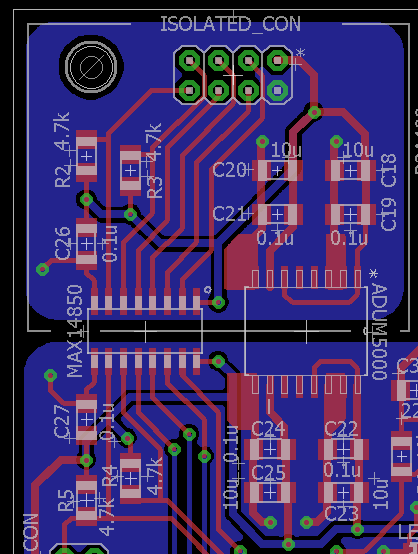
\includegraphics[width=0.5\textwidth, angle=90]{Chapter_3/PV_MeasPCB_ZOOM_ISO.PNG}
		\rule{35em}{0.5pt}
	\caption{Isolation layout as shown in Eagle board environment}
	\label{fig:PV_MeasPCB_ZOOM_ISO}
\end{figure}

The different ground plane of the "isolated area" is the first thing noticed here, with a very simple explanation. The whole isolation circuit will be totally useless if we shorted the two parts' grounds together because the isolation of two systems require the separation of both power traces, the positive voltage line but the ground too.

For safety reasons we also kept the two sides of the isolation layer as far away as possible, leaving a significant gap in the line crossing the two isolation ICs. Lastly, it is interesting to mention the enlarged pads for the ground pins of the isolated DC-DC converter chip. The ADuM5000 is a power device that dissipates approximately 1 W of power when fully loaded. Because it is not possible to apply a heat sink to an isolation device, the device primarily depends on heat dissipation into the PCB through the ground pins, hence the enlarged design.

One more thing to mention concerning the design of the board is the width of the copper traces. Except from the traces that the main current of the PV module flows, there are only two values used. All normal signal traces are 0.4064mm wide and all power lines, for both 5V and 3.3V, are 0.6096mm wide. In the figure -FIGURE NUMBER- are highlighted all power lines inside the board's layout.\\


\begin{figure}[htbp]
	\centering
	\begin{subfigure}[b]{.45\textwidth}
		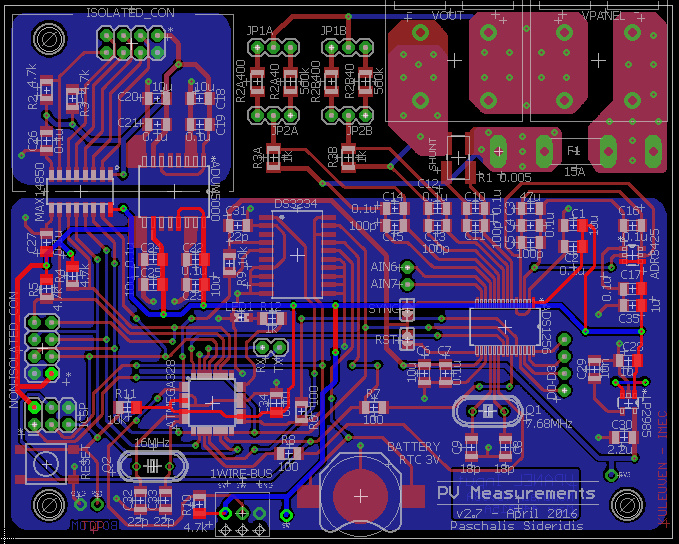
\includegraphics[width=\textwidth]{Chapter_3/PV_MeasPCB_5V.PNG}
	    \caption[]{5V power line}
	    \label{fig:PV_MeasPCB_5V}
	\end{subfigure}
    ~
	\begin{subfigure}[b]{.45\textwidth}
		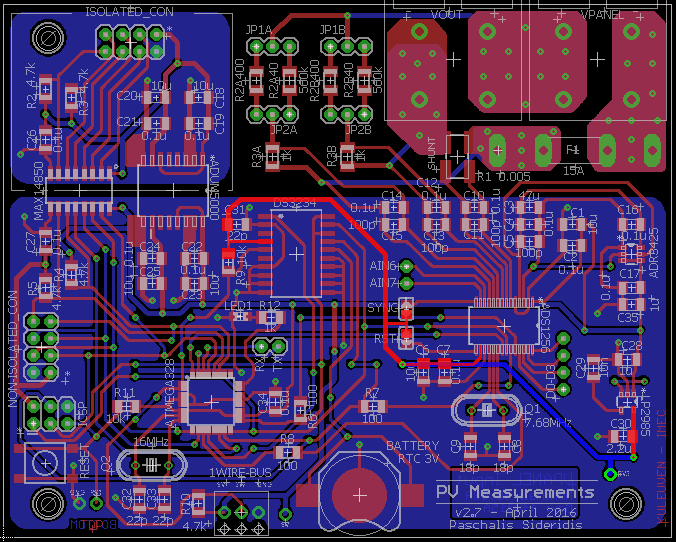
\includegraphics[width=\textwidth]{Chapter_3/PV_MeasPCB_3V3.PNG}
	    \caption[]{3.3V power line}
	    \label{fig:PV_MeasPCB_3V3}
	\end{subfigure}
	\rule{35em}{0.5pt}
	\caption{PV Measurement PCB power lines}
	\label{fig:PV_MeasPCB_powerLines}
\end{figure}

Last factor that is crucial to underline is a modification we had to make to the fabricated boards. The PV Measurement PCB was initially designed to work with a control device such as the Arduino Uno board we used during prototyping, which operates on 5V logic. But, as we will describe in more depth later on the report, we decided to use a control device with 3.3V logic, so a minor modification was needed to the PCB. More on that subject will be discussed in the next section.

\subsubsection{Assembly and Testing}
After the design of the physical layout for the measurement board, it is time for the fabrication of the PCBs, the assembly and soldering of the components and last but not least the boards' testing. As we have already discussed, we decide to get the PCBs fabricated by a manufacturer company and therefore there are not a lot of things to describe concerning this process. So, let start from the moment that the PCBs came already fabricated, as shown in the figure -FIGURE NUMBER-.\\


\begin{figure}[htbp]
	\centering
		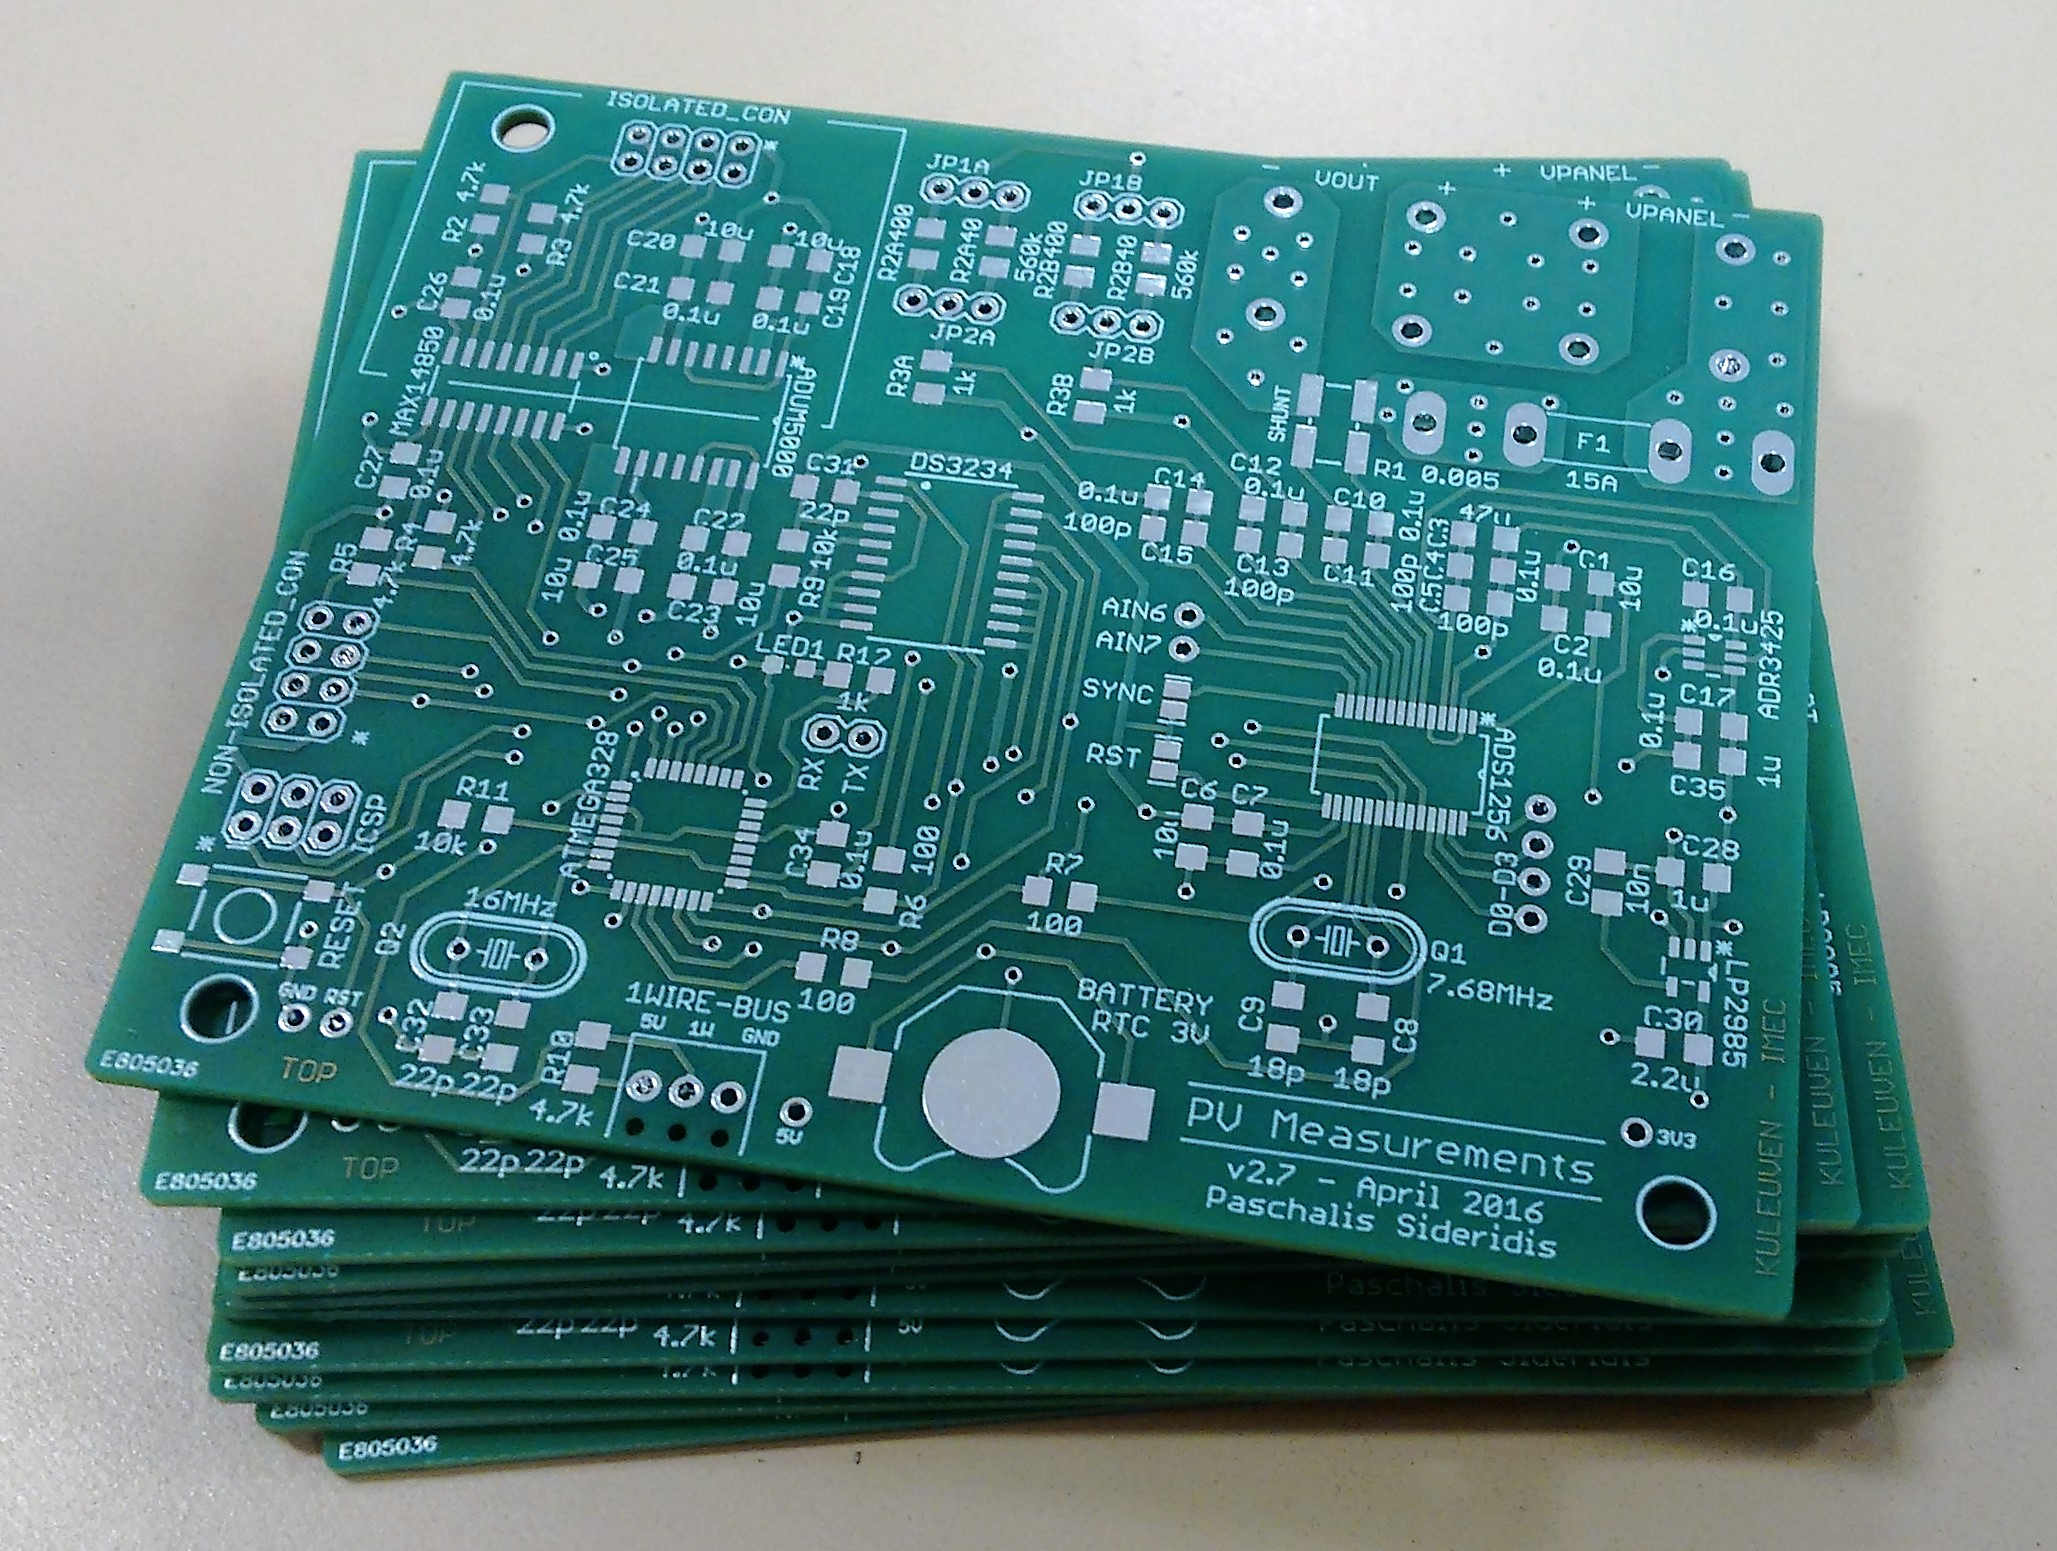
\includegraphics[width=0.7\textwidth]{Chapter_3/PCB_stack.jpg}
		\rule{35em}{0.5pt}
	\caption{Stack of fabricated PCBs}
	\label{fig:PCB_stack}
\end{figure}

At this point the board is just a single circuit, without any components, and as a result not capable of any functionality. In order to create a working device we need to assemble the PCB, which actually means the soldering of all parts and hardware to the board. There are a few different techniques of soldering electronic components onto a PCB, sometimes depending on the type of the parts (through hole or surface mounted) or the production volume, but the most popular solutions for a small batch of boards are based on the use of:

\begin{itemize}
    \item Soldering iron
    \item Hot air gun
    \item Reflow oven
\end{itemize}

In our case, we used the combination of the first two methods and the final result of the assembled PV Measurement PCB is shown in the figure -FIGURE NUMBER-. More information about the soldering process of the PCBs is given in the Appendix chapter.\\


\begin{figure}[htbp]
	\centering
		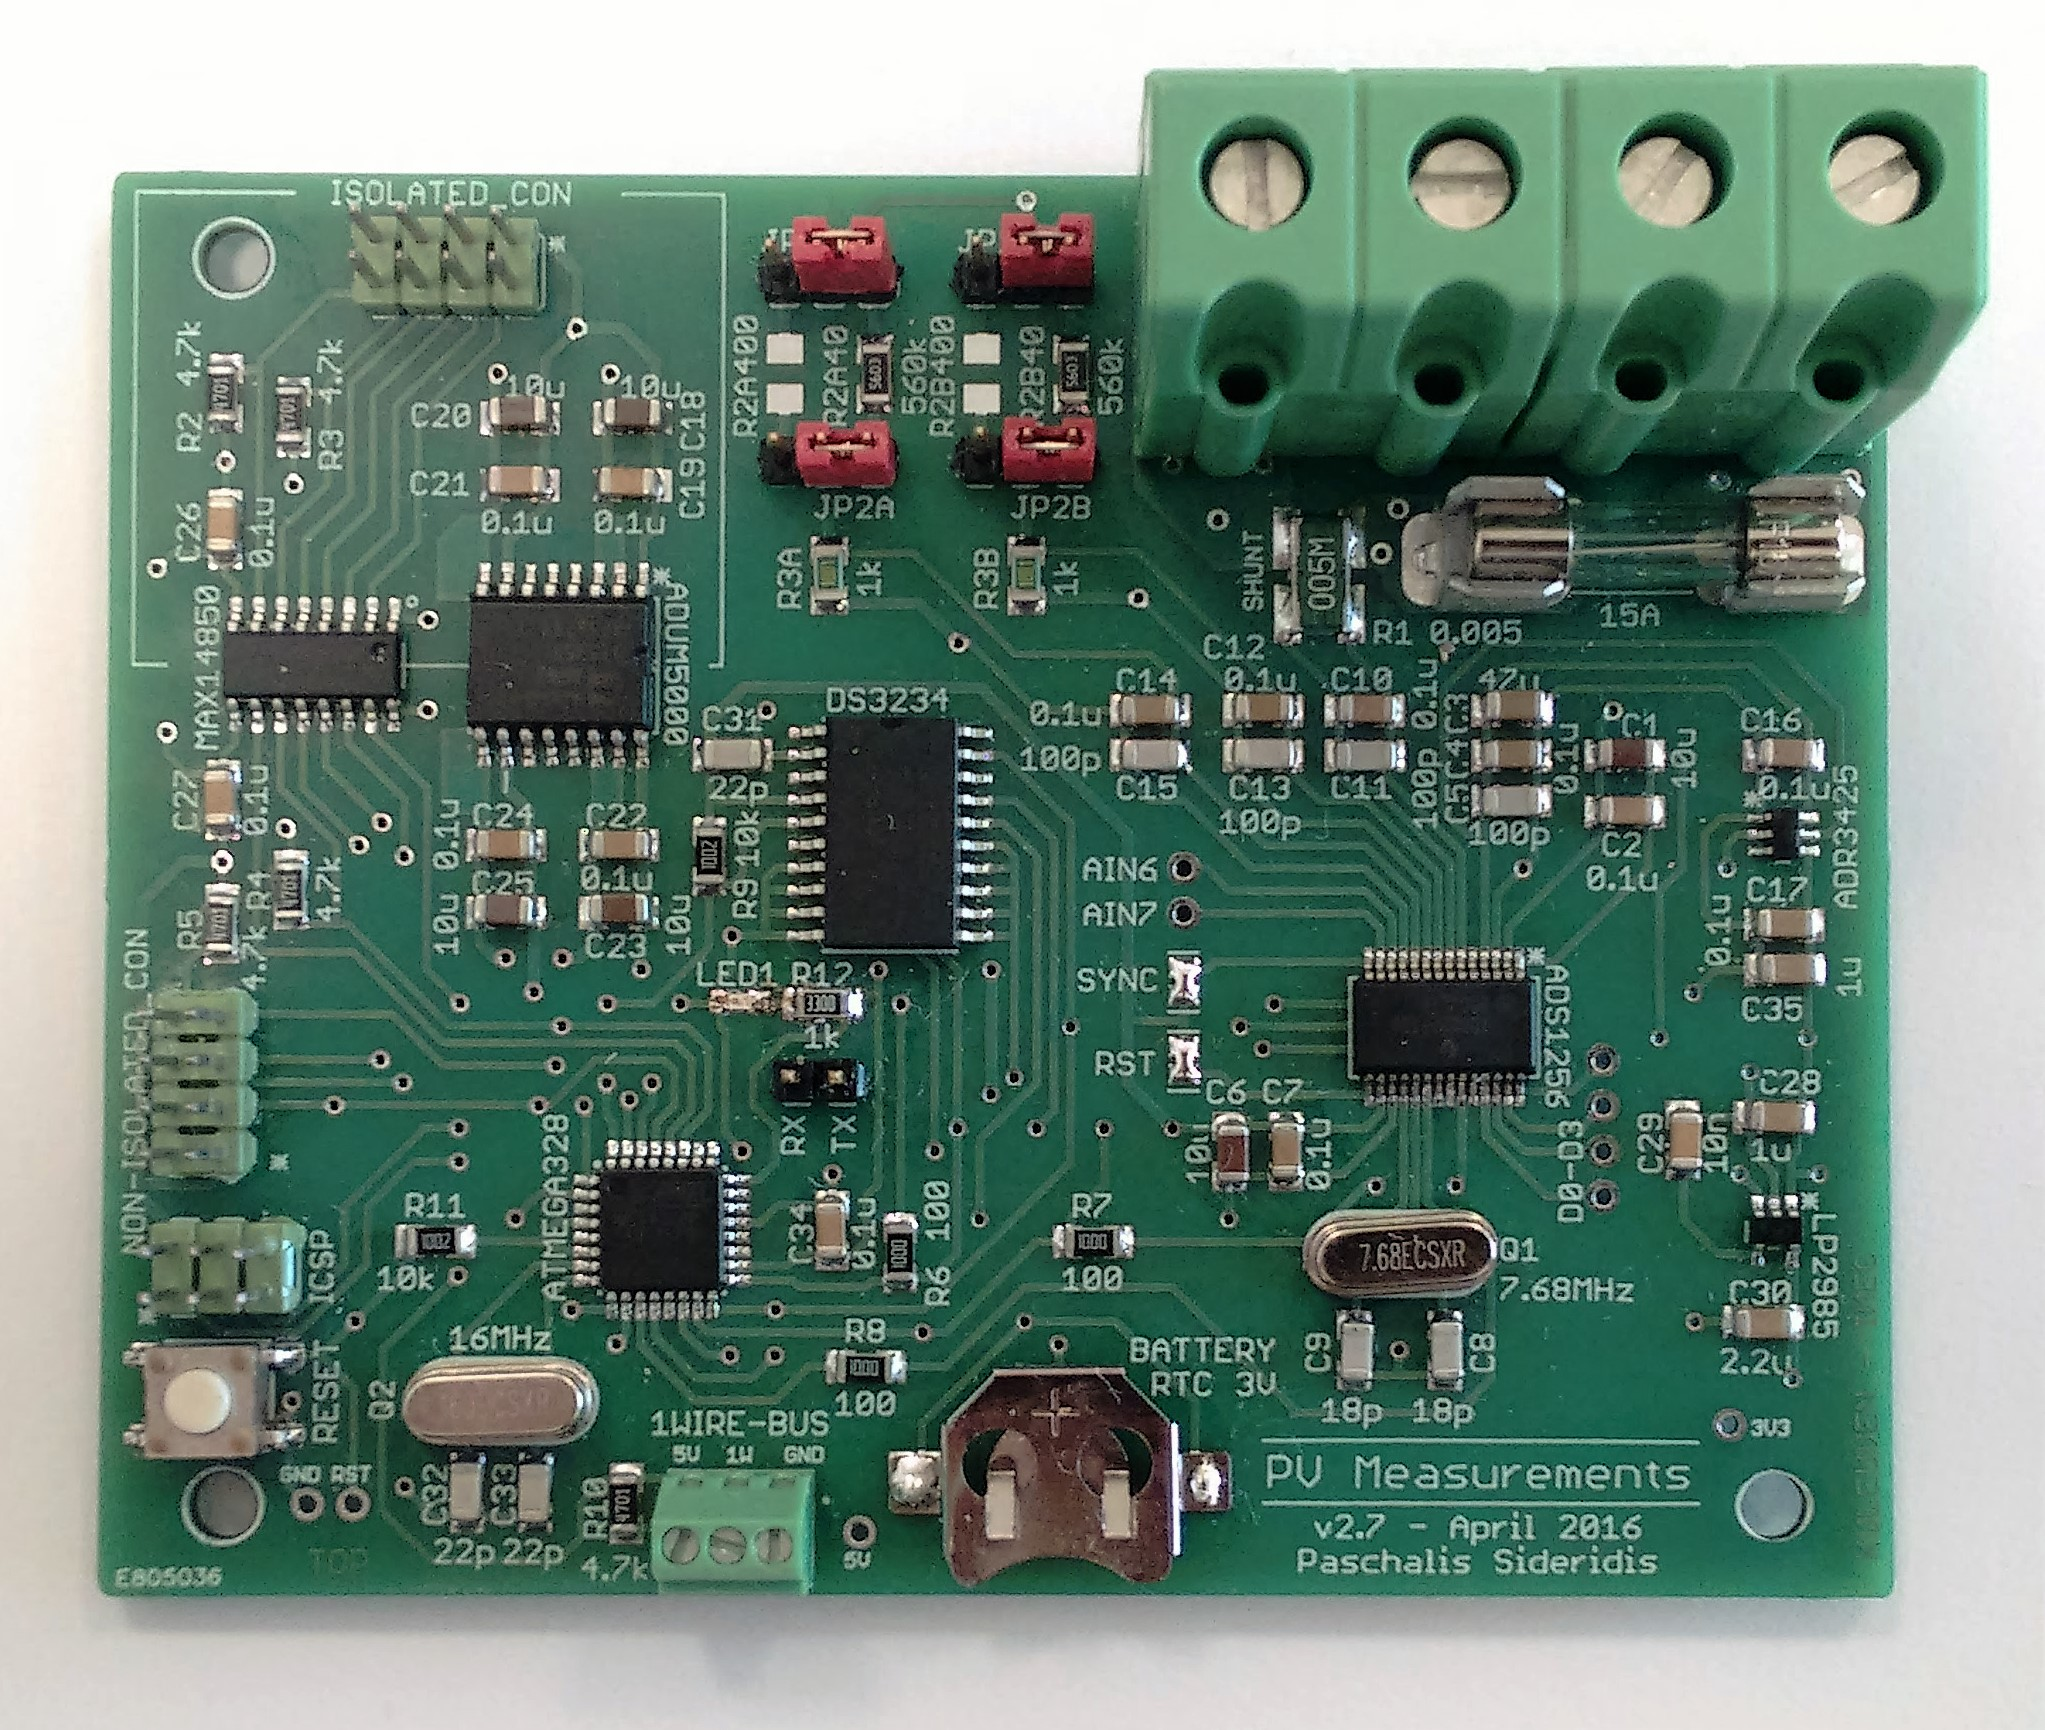
\includegraphics[width=.95\textwidth]{Chapter_3/PV_MeasurementPCB_assembled.jpg}
		\rule{35em}{0.5pt}
	\caption{Assembled PV Measurement PCB}
	\label{fig:PV_MeasurementPCB_assembled}
\end{figure}

The last step of the whole PCB design and fabrication process is the crucial stage of testing. 

Usually we start with the very basics and gradually included more sophisticated routines to the testing procedure. In particular, when a PCB was fully assembled, we carry out the following three checks in this particular order: 

%\begin{enumerate}
%    \item Visual check, making sure that all solder points are looking clean without solder bridges and shorts
%    \item Simple blink LED script programing to the microcontroller, to ensure that the microco 
%    \item 
%\end{enumerate}
